% Priručnik: procjena eksponenta alpha u transportnom DEB-u (tDEB)
% Prevođenje: pdflatex prirucnik_alfa.tex (dva prolaza)
\documentclass[11pt,a4paper]{article}
\usepackage[T1]{fontenc}
\usepackage[utf8]{inputenc}
\usepackage[croatian]{babel}
\usepackage{amsmath,amssymb}
\usepackage{libertinus-type1}
\usepackage{libertinust1math}
\usepackage{newunicodechar}
\newunicodechar{≈}{\ensuremath{\approx}}
\newunicodechar{≤}{\ensuremath{\le}}
\newunicodechar{≥}{\ensuremath{\ge}}
\newunicodechar{↔}{\ensuremath{\leftrightarrow}}
\newunicodechar{−}{\ensuremath{-}}
\newunicodechar{α}{\ensuremath{\alpha}}
\newunicodechar{β}{\ensuremath{\beta}}
\newunicodechar{κ}{\ensuremath{\kappa}}
\newunicodechar{Δ}{\ensuremath{\Delta}}
\newunicodechar{χ}{\ensuremath{\chi}}
\newunicodechar{λ}{\ensuremath{\lambda}}
\usepackage{microtype}
\usepackage[a4paper,top=2.4cm,bottom=2.5cm,left=2.4cm,right=2.4cm,headheight=14pt]{geometry}
\usepackage{booktabs,tabularx,longtable,array,makecell}
\usepackage{graphicx}
\usepackage[dvipsnames,table]{xcolor}
\usepackage[most]{tcolorbox}
\usepackage[inline]{enumitem}
\usepackage{titlesec}
\usepackage{needspace}
\newcommand{\sectionbreak}{\needspace{12\baselineskip}}
\newcommand{\subsectionbreak}{\needspace{6\baselineskip}}
\usepackage{fancyhdr}
\usepackage[font=small,labelfont={bf,sf},labelsep=period]{caption}
\usepackage{tikz}
\usetikzlibrary{arrows.meta,positioning,calc,shapes.geometric,babel}
\usepackage{csquotes}
\usepackage[hidelinks]{hyperref}

\definecolor{akcent}{HTML}{1F4E79}
\definecolor{akcent2}{HTML}{C51B7D}
\definecolor{siva}{HTML}{5A5A5A}
\definecolor{svijetla}{HTML}{F3F6FA}
\definecolor{zelena}{HTML}{1B9E77}

\titleformat{\section}{\sffamily\Large\bfseries\color{akcent}}{\thesection}{0.7em}{}
\titleformat{\subsection}{\sffamily\large\bfseries\color{akcent}}{\thesubsection}{0.6em}{}
\titleformat{\subsubsection}{\sffamily\normalsize\bfseries}{\thesubsubsection}{0.5em}{}
\titlespacing*{\section}{0pt}{1.6em}{0.7em}
\titlespacing*{\subsection}{0pt}{1.2em}{0.5em}

\pagestyle{fancy}
\fancyhf{}
\fancyhead[L]{\sffamily\small\color{siva}Procjena eksponenta $\alpha$ u transportnom DEB-u}
\fancyhead[R]{\sffamily\small\color{siva}AdvanDEB · radni priručnik}
\fancyfoot[C]{\sffamily\small\thepage}
\renewcommand{\headrulewidth}{0.4pt}

\setlist{itemsep=0.25em,topsep=0.4em}
\setlength{\parskip}{0.35em}
\setlength{\parindent}{0pt}
\renewcommand{\arraystretch}{1.18}

\newcommand{\GrowthMaxDiff}{6}
\newcommand{\ProfLonlyMax}{2{,}12}
\newcommand{\CIlo}{0{,}60}
\newcommand{\CIhi}{0{,}85}
\newcommand{\AlphaBestProf}{0{,}700}
\newcommand{\ICtwoThirdsLo}{0{,}40}
\newcommand{\ICtwoThirdsHi}{0{,}44}
\newcommand{\IConeLo}{0{,}61}
\newcommand{\IConeHi}{0{,}74}
\newcommand{\NaiveBiasMin}{0{,}07}
\newcommand{\NaiveBiasMax}{0{,}11}
\newcommand{\MCreps}{40}
\newcommand{\MCAsevenfiveMed}{0{,}81}
\newcommand{\MCAsevenfiveLo}{0{,}50}
\newcommand{\MCAsevenfiveHi}{1{,}20}
\newcommand{\MCArmse}{0{,}30}
\newcommand{\MCBrmse}{0{,}07}
\newcommand{\MCCrmse}{0{,}11}
\newcommand{\MCDrmse}{0{,}07}
\newcommand{\MCErmse}{0{,}03}
\newcommand{\MCFrmse}{0{,}03}
\newcommand{\MCCmisMed}{0{,}685}
\newcommand{\MCCokMed}{0{,}763}
\newcommand{\MCFmisMed}{0{,}693}
\newcommand{\MCFokMed}{0{,}751}

\makeatletter\let\inputtab\@@input\makeatother

% ---- notacija
\newcommand{\pd}{\dot{p}}
\newcommand{\pAm}{\{\dot p_{Am}\}}
\newcommand{\pM}{[\dot p_M]}
\newcommand{\EG}{[E_G]}
\newcommand{\Vref}{V_{\mathrm{ref}}}
\newcommand{\dc}{{,}}

% ---- okviri za izjave
\newtcolorbox{kljucno}[1][]{enhanced,breakable,colback=svijetla,colframe=akcent,boxrule=0.6pt,arc=2pt,
  left=8pt,right=8pt,top=6pt,bottom=6pt,fonttitle=\sffamily\bfseries,title=#1}
\newtcolorbox{upozorenje}[1][]{enhanced,breakable,colback=akcent2!5,colframe=akcent2,boxrule=0.6pt,arc=2pt,
  left=8pt,right=8pt,top=6pt,bottom=6pt,fonttitle=\sffamily\bfseries,title=#1}
\newtcolorbox{propozicija}[1]{enhanced,breakable,colback=white,colframe=zelena,boxrule=0.6pt,arc=2pt,
  left=8pt,right=8pt,top=5pt,bottom=5pt,fonttitle=\sffamily\bfseries,coltitle=white,colbacktitle=zelena,title=#1}

% oznake izjava: H (hipoteza), T (literatura), E (empirija), P (propozicija), S (simulacija)
\newcommand{\izjava}[2]{\par\noindent\hangindent=2.6em\hangafter=1\makebox[2.6em][l]{\sffamily\bfseries\color{akcent}#1}#2\par\vspace{0.25em}}
\newcommand{\zaalfa}[1]{\par\noindent\hangindent=2.6em\hangafter=0\hspace*{2.6em}{\sffamily\small\bfseries\color{zelena}Za $\alpha$:} #1\par\vspace{0.45em}}
\newcommand{\pouzd}[1]{{\sffamily\scriptsize\color{siva}[#1]}}

\hypersetup{pdftitle={Procjena eksponenta alfa u transportnom DEB-u},pdfauthor={AdvanDEB},pdflang={hr}}

\begin{document}

\begin{titlepage}
\thispagestyle{empty}
\vspace*{1.2cm}
{\sffamily\small\color{akcent}\MakeUppercase{AdvanDEB · radni priručnik}}\par
\vspace{0.6cm}
{\sffamily\bfseries\fontsize{28}{33}\selectfont\color{akcent} Procjena eksponenta $\boldsymbol{\alpha}$\\[2pt] u transportnom DEB-u\par}
\vspace{0.5cm}
{\Large Teorija, podaci i protokol za procjenu\\ morfologije transportne mreže\par}
\vspace{0.9cm}
{\color{siva}\rule{\linewidth}{0.5pt}}
\vspace{0.3cm}

\begin{tabularx}{\linewidth}{@{}lX@{}}
\textbf{Verzija} & 1.0 (radna) · 3. studenoga 2026. \\
\textbf{Temelji} & Pregled literature teorije dinamičkih energijskih proračuna (DEB) i teorije metaboličkog skaliranja (MTE); analitičke propozicije izvedene u priručniku (Dodatak A); simulacije minimalnog modela (Dodatak B). \\
\textbf{Namjena} & Zajednički radni dokument za odabir vrsta, prikupljanje podataka i procjenu $\alpha$ u transportnom DEB-u (tDEB). \\
\end{tabularx}

\vspace{0.6cm}
\begin{kljucno}[Kako čitati ovaj priručnik]
Svaka tvrdnja ima oznaku koja kaže odakle dolazi i kako se može provjeriti.
\begin{itemize}[leftmargin=4.2em,labelwidth=3.4em,align=left]
\item[\textbf{H}] hipoteza ili pretpostavka modela koju priručnik testira; uz svaku je navedeno gdje se testira (propozicija, simulacija ili korak protokola);
\item[\textbf{T}] tvrdnja iz objavljene literature, izrečena vlastitim riječima, s izvorom;
\item[\textbf{E}] empirijski podatak (izmjereni eksponent) s izvorom;
\item[\textbf{P}] propozicija izvedena u ovom priručniku (izvodi u Dodatku A);
\item[\textbf{S}] rezultat simulacije (kod i postavke u Dodatku B).
\end{itemize}
Ostalo je ili izvod u samom tekstu ili je izričito navedeno kao pretpostavka modela. Pouzdanost literaturnog podatka označena je u uglatim zagradama: \pouzd{puni tekst}, \pouzd{sažetak} ili \pouzd{izvedeno}. Bibliografski podaci provjereni su u PubMedu i Crossrefu.
\end{kljucno}

\vfill
{\small\color{siva} Dokument je priređen za projekt AdvanDEB uz pomoć Claudea (Anthropic): pregled i provjera literature, izvodi propozicija i simulacije. Sve brojke iz simulacija generirane su skriptama u \texttt{docs/alpha-handbook/sim/} i mogu se reproducirati.\par}
\end{titlepage}

{\small\setlength{\parskip}{0pt}\tableofcontents}
\clearpage

\section{Ukratko}

\begin{kljucno}[Osam poruka za brzo čitanje]
\begin{enumerate}[leftmargin=1.6em]
\item \textbf{Što je $\alpha$.} $\alpha$ je eksponent kojim efektivni kapacitet izmjene između transportnog kompartimenta i tkiva raste sa \emph{strukturnim} volumenom, $A\propto V^{\alpha}$. Kapacitet izmjene je površina × gustoća transportera × propusnost (H2). $\alpha$ \emph{nije} metabolički eksponent $b$ (pogl.~\ref{sec:definicija}, \ref{sec:zamke}).
\item \textbf{Raspon.} Raspon $2/3\le\alpha\le1$ dobar je radni prior za odrasle organizme s unutarnjom mrežom, ali nije zakon. Vrijednosti ispod $2/3$ zabilježene su, a iznad $1$ javljaju se prolazno, dok se mreža gradi (T11, E3, E4).
\item \textbf{MTE ne daje $\alpha=1$.} Prema West–Brown–Enquistu (WBE) $M^{3/4}$ je \emph{gornja} granica efektivne površine izmjene fraktalne mreže koja ispunjava volumen. Prema 1 se eksponent približava tek uz čisto Poiseuilleovo grananje (T8, T9). Ni fraktalna dimenzija izmjerena na plošnim slikama mreže ne daje $\alpha=1$ (H4, P6).
\item \textbf{Morfometrija daje prior, ne procjenu.} Izmjerene površine izmjene kod sisavaca skaliraju s eksponentom $0{,}87$–$0{,}99$, iznad WBE granice. Prate vršnu potražnju za kisikom, a ne bazalni metabolizam (E1, E2).
\item \textbf{Rast nikad nije dovoljan.} Uz brz transportni kompartiment somatski tok je $\kappa\,\pd_A$ s $\kappa=\beta_S/(\beta_S+\beta_R)$, a $L_\infty$ ne ovisi o $\alpha$ (P1). U Monte Carlu procjene iz same krivulje rasta raspršene su po cijelom dopuštenom rasponu (za istinski $\alpha=0{,}75$ 10.–90. percentil je \MCAsevenfiveLo–\MCAsevenfiveHi, a RMSE do \MCArmse; S2, S6).
\item \textbf{Gladovanje je najinformativnije, spremište drugo.} Specifična brzina pražnjenja spremišta pri gladovanju skalira kao $V^{\alpha-1}$ i ne ovisi o eksponentu asimilacije $a$ (P3). Serija gladovanja u tri veličine daje RMSE do \MCErmse, najbolje od svih dizajna. Gustoća spremišta po strukturi skalira kao $V^{a-\alpha}$ (P2) i uz 8–16 mjerenja daje RMSE do \MCBrmse–\MCCrmse{}, ovisno o mjernoj pogrešci (S6).
\item \textbf{Pogrešan $a$ spušta $\hat\alpha$.} Ako je stvarni $a=0{,}72$, a fit pretpostavlja $2/3$, medijan $\hat\alpha$ pada s \MCCokMed{} na \MCCmisMed{} (samo spremište) i s \MCFokMed{} na \MCFmisMed{} (spremište i gladovanje), u skladu s $\hat\alpha\approx\alpha-(a-2/3)$ iz P2 (S6). Pristranost ostaje i uz gladovanje, pa unos hrane prema veličini treba mjeriti.
\item \textbf{Protokol:} prior iz tipa mreže → gladovanje prema veličini, spremište po strukturi prema veličini i unos hrane prema veličini → zajednički fit dinamičkog modela s profilom vjerodostojnosti → filogenetski test (H6; pogl.~\ref{sec:protokol}). Nagib spremišta ne čitati „na oko“: naivna formula podcjenjuje $\alpha$ za \NaiveBiasMin–\NaiveBiasMax{} (S4).
\end{enumerate}
\end{kljucno}

\section{Što je $\alpha$}\label{sec:definicija}

\subsection{Polazna jednadžba: kinetika izmjene kroz sučelje}\label{sec:polazna}

Transportni DEB (tDEB) razlikuje transportni kompartiment (krv, hemolimfa) s energijom $E_T$ i spremište (storage, npr.\ lipidi u masnom tkivu) s energijom $E_E$. Energija između njih prelazi kroz sučelje veličine $A$. Izmjenu opisujemo trima pretpostavkama modela.

\textbf{Pretpostavka modela 1: djelovanje masa.} Tok iz kompartimenta proporcionalan je koncentraciji energije u kompartimentu iz kojeg izlazi i veličini sučelja kroz koje prolazi:
\begin{equation}
\pd_{TE}=k_{TE}\,\frac{E_T}{V_T}\,A,\qquad \pd_{ET}=k_{ET}\,\frac{E_E}{V_E}\,A .
\end{equation}
Ovdje je $\pd_{TE}$ tok iz transporta u spremište, $\pd_{ET}$ tok u suprotnom smjeru, a $k_{TE}$ i $k_{ET}$ su konstante brzine po jedinici sučelja.

\textbf{Pretpostavka modela 2: zajednički volumen.} Oba kompartimenta raspoređena su po cijelom tijelu, pa se koncentracije računaju prema istom strukturnom volumenu, $V_T=V_E=V$. Veličina sučelja skalira kao $A=V^{\alpha}$; to je definicija eksponenta $\alpha$ (pogl.~\ref{sec:radna}).

\textbf{Pretpostavka modela 3: isti transporteri, različit broj.} Pojedini transporter prenosi energiju istom brzinom u oba smjera, a smjerovi se razlikuju samo brojem transportera. Tada je $k_{TE}=\beta_G$ i $k_{ET}=k_E\beta_G$, gdje je $k_E$ omjer broja transportera koji prenose energiju iz spremišta u transport i broja onih koji je prenose iz transporta u spremište.

Neto tok iz transporta u spremište tada je
\begin{equation}\label{eq:ploca}
\Delta\pd=\pd_{TE}-\pd_{ET}=\beta_G\,\frac{E_T-k_E E_E}{V}\,V^{\alpha}
\quad\Rightarrow\quad
\boxed{\;\Delta\pd=\beta_G\,(E_T-k_E\,E_E)\,V^{\alpha-1}\;}
\end{equation}
Iz jednadžbe~\eqref{eq:ploca} odmah slijede tri svojstva:
\begin{itemize}
\item Izmjena staje ($\Delta\pd=0$) pri $E_T=k_E E_E$. Omjer broja transportera $k_E$ dakle određuje ravnotežni omjer energije u transportu i spremištu: uz mali $k_E$ transport sadrži malen dio energije spremišta.
\item $\beta_G$ je sposobnost transporta po jedinici sučelja i ponaša se kao conductance. Njegove jedinice ovise o $\alpha$ (pogl.~\ref{sec:normalizacija}).
\item Specifična brzina izmjene $\Delta\pd/E$ skalira kao $V^{\alpha-1}$. Uz $\alpha<1$ veći organizam sporije izmjenjuje svoje zalihe, a uz $\alpha=1$ brzina ne ovisi o veličini (P3).
\end{itemize}
Za izmjenu sa spremištem u modelu je $\beta_G=\beta_E$. Istim su oblikom, ali bez povratnog toka, opisani tokovi iz transporta u strukturu ($\beta_S$) i u reprodukciju ($\beta_R$); slika~\ref{fig:shema} prikazuje sve tokove, a potpuni model dan je jednadžbama~\eqref{eq:mT}–\eqref{eq:mV}. Faktor $V^{\alpha-1}$ u modelu se koristi u normaliziranom obliku, $r(V)\propto V^{\alpha-1}$ (jedn.~\eqref{eq:norm}). Standardni DEB polazi od srodne ideje: mobilizacija rezerve proporcionalna je površini sučelja između rezerve i strukture (Marques i sur. 2018).

\begin{figure}[ht]
\centering
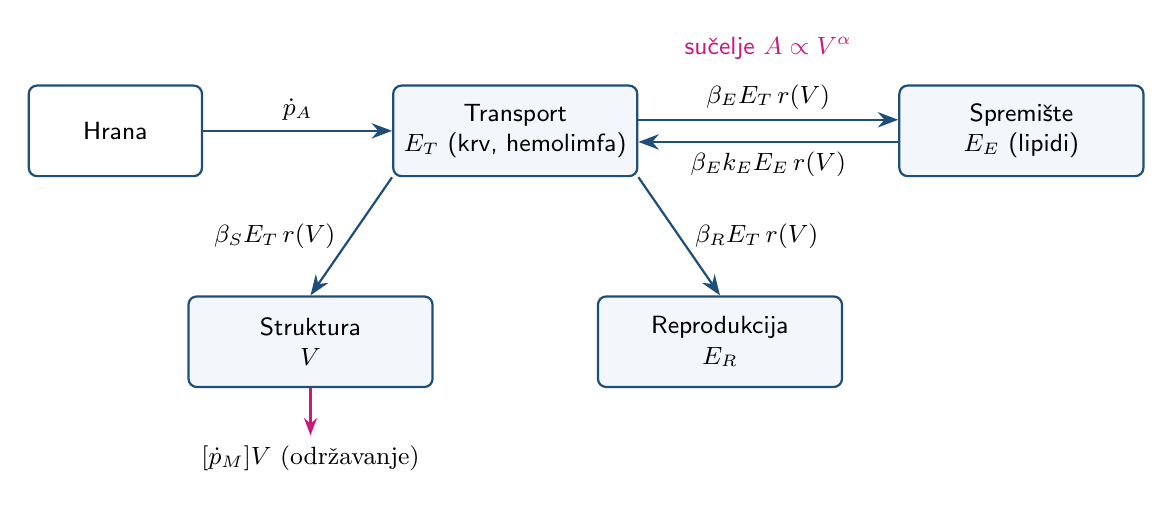
\begin{tikzpicture}[
  komp/.style={draw=akcent,thick,rounded corners=3pt,minimum width=3.1cm,minimum height=1.15cm,align=center,font=\sffamily\small,fill=svijetla},
  tok/.style={-{Stealth[length=2.6mm]},thick,color=akcent},
  lab/.style={font=\small,color=black}]
\node[komp] (T) {Transport\\ $E_T$ (krv, hemolimfa)};
\node[komp,right=3.3cm of T] (E) {Spremište\\ $E_E$ (lipidi)};
\node[komp,below=1.5cm of T,xshift=-2.6cm] (V) {Struktura\\ $V$};
\node[komp,below=1.5cm of T,xshift=2.6cm] (R) {Reprodukcija\\ $E_R$};
\node[komp,left=2.4cm of T,minimum width=2.2cm,fill=white] (H) {Hrana};
\draw[tok] (H) -- node[above,lab]{$\pd_A$} (T);
\draw[tok] ([yshift=4pt]T.east) -- node[above,lab]{$\beta_E E_T\,r(V)$} ([yshift=4pt]E.west);
\draw[tok] ([yshift=-4pt]E.west) -- node[below,lab]{$\beta_E k_E E_E\,r(V)$} ([yshift=-4pt]T.east);
\draw[tok] (T.south west) -- node[left,lab,xshift=-2pt]{$\beta_S E_T\,r(V)$} (V.north);
\draw[tok] (T.south east) -- node[right,lab,xshift=2pt]{$\beta_R E_T\,r(V)$} (R.north);
\draw[-{Stealth[length=2.2mm]},thick,color=akcent2] (V.south) -- ++(0,-0.6) node[below,lab]{$\pM V$ (održavanje)};
\node[font=\small\sffamily,color=akcent2,align=center] at ($(T)!0.5!(E)+(0,1.05)$) {sučelje $A\propto V^{\alpha}$};
\end{tikzpicture}
\caption{Minimalni transportni DEB koji se koristi u ovom priručniku. Svi tokovi iz transporta prolaze kroz sučelje čija veličina skalira kao $V^{\alpha}$; faktor $r(V)\propto V^{\alpha-1}$ definiran je jednadžbom~\eqref{eq:norm}. Pretpostavka modela: održavanje strukture $\pM V$ plaća se iz somatskog toka prije rasta (jedn.~\eqref{eq:mV}).}
\label{fig:shema}
\end{figure}

\subsection{Pretpostavke i hipoteze o $\alpha$}\label{sec:hipoteze}

Sljedeće hipoteze određuju kako se $\alpha$ tumači i mjeri. Nijedna nije dokazana. Uz svaku je navedeno gdje se u priručniku testira.

\izjava{H1}{\textbf{Granični slučajevi.} $\alpha=1$ znači da svaka stanica leži izravno uz transportnu mrežu, pa kapacitet izmjene raste proporcionalno volumenu. $\alpha<1$ znači da je izravno uz mrežu samo dio stanica, a ostale se opskrbljuju difuzijom kroz intersticij. \emph{Testira se:} geometrijski, jedn.~\eqref{eq:D3} i P6; mjerno, morfometrijom površine izmjene po jedinici volumena (Korak 3).}
\izjava{H2}{\textbf{Generalizirana površina.} $A$ nije samo geometrijska površina. Obuhvaća broj receptora i transportera, propusnost sučelja, difuziju kroz intersticij i nejednak tlak u mreži, a dio tih učinaka može se pripisati i $\beta$. Difuzija kroz intersticij tretira se kao kašnjenje, a ne kao glavni put transporta, pa u minimalnom modelu nema vlastiti član. \emph{Testira se:} usporedbom procjene $\hat\alpha$ s morfometrijskim eksponentom (Korak 5). Razlika upućuje na gustoću transportera ili propusnost.}
\izjava{H3}{\textbf{$\alpha$ pripada mreži, a ne kompartimentu.} $\alpha$ je svojstvo morfologije transportne mreže, pa svi tokovi iz transporta dijele isti $\alpha$. Razlike među kompartimentima (spremište, struktura, reprodukcija) ulaze u $\beta_E$, $\beta_S$ i $\beta_R$. Radna gornja granica za izgrađenu mrežu je $\alpha\le1$; prolazne vrijednosti iznad 1 dok se mreža gradi (E4) izvan su ove hipoteze. \emph{Testira se:} zajednički $\alpha$ ugrađen je u model kao pretpostavka (jedn.~\eqref{eq:mT}–\eqref{eq:mV}). Gornja granica se pri fitanju ne nameće (S6, Korak 4), pa je interval pouzdanosti iznad 1 dokaz protiv nje.}
\izjava{H4}{\textbf{Argument fraktalne dimenzije.} Vaskularne mreže kojima je na plošnim (2D) slikama izmjerena fraktalna dimenzija oko 1,3–1,7 ponekad se uzimaju kao dokaz da je $\alpha=1$, tj. da površina izmjene raste proporcionalno volumenu. \emph{Testira se:} P6. Ishod: dimenzija $D$ izmjerena u ravnini daje $\alpha_{2D}=D/2=0{,}65$–$0{,}85$, a ne 1, jer $\alpha=1$ traži mrežu koja ispunjava prostor. Literaturne vrijednosti fraktalne dimenzije navedene su u pogl.~\ref{sec:teorija}.}
\izjava{H5}{\textbf{Dvije mreže.} Energija i kisik mogu imati različit $\alpha$ ako ih raznose različite mreže. Kod kukaca kisik dolazi trahejama, a energija hemolimfom; kod vodozemaca dio kisika ulazi kroz kožu. Ograničavajuća tada može postati ona mreža čiji kapacitet sporije raste s veličinom. \emph{Testira se:} u Koraku 0 kisik se tretira zasebno ($\alpha_{O_2}$), a kukci su prirodan test (T6; pogl.~\ref{sec:vrste}). Sprezanje dviju mreža u modelu otvoreno je pitanje (pogl.~\ref{sec:otvoreno}).}
\izjava{H6}{\textbf{Filogenetska očuvanost.} $\alpha$ je svojstvo tipa mreže ili klade, pa srodne vrste imaju sličan $\alpha$. Ako to vrijedi, $\alpha$ se za vrstu bez podataka može preuzeti od srodnih vrsta umjesto da se fita. \emph{Testira se:} Korak 6 (PGLS među tipovima mreža, Pagelov $\lambda$, Blombergov $K$).}
\izjava{H7}{\textbf{Spremište mladih i odraslih otkriva $\alpha$.} Gustoća spremišta po strukturi mijenja se s veličinom ovisno o $\alpha$: uz $a=2/3$ i $\alpha=1$ mladi su deblji od odraslih, a uz $\alpha=2/3$ nisu. Mjerenjem spremišta kod mladih i odraslih može se dakle procijeniti $\alpha$, ako je spremište izraženo po strukturi, a ne po ukupnoj masi (pretvorba u Koraku 3). \emph{Testira se:} P2 (kvazi-ravnotežna gustoća $\propto V^{a-\alpha}$), S1 (dinamika rasta), S4 (pristranost naivnog čitanja nagiba) i S5 (osjetljivost na početne uvjete).}
\izjava{H8}{\textbf{Ograničena homeostaza.} Pri stalnoj hrani omjer spremišta i strukture ne bi se smio drastično mijenjati tijekom ontogeneze. To je zahtjev biološke uvjerljivosti, a ne izmjereni podatak. \emph{Testira se:} P2 pokazuje posljedicu: gustoća spremišta ne ovisi o veličini samo uz $a\approx\alpha$, pa uz $\alpha=1$ hipoteza traži da i asimilacija skalira približno s volumenom. Za pojedinu vrstu provjerava se u Koraku 5.}
\izjava{H9}{\textbf{$\alpha$ i tip rasta.} $\alpha\neq1$ mogao bi se poklapati s indeterminiranim rastom. Minimalni model to ne reproducira: $L_\infty$ ne ovisi o $\alpha$ (P1), a uz ograničen protok granicu veličine postavlja upravo $\alpha<1$ (P5). Hipoteza zato ostaje otvorena. \emph{Testira se:} Korak 6 na skupu vrsta; vidi i pogl.~\ref{sec:otvoreno}.}

\textbf{Ograda modela: kvazi-ravnoteža.} Propozicije P1–P3 pretpostavljaju da je izmjena između transporta i ostalih kompartimenata brza u odnosu na rast; u P1 i P2 to znači $E_T\approx k_E E_E$. Kod mladih, koji relativno brže rastu, spremište zaostaje za tom ravnotežom. Kvazi-ravnoteža zato dobro opisuje odrasle, a kod mladih daje pristrane nagibe gustoće spremišta (S4). Zbog toga se $\alpha$ procjenjuje fitanjem dinamičkog modela (Korak 4), a ne formulama kvazi-ravnoteže.

\subsection{Radna definicija}\label{sec:radna}

Na temelju jedn.~\eqref{eq:ploca} i hipoteza H1–H3 predlažemo ovu radnu definiciju:

\begin{kljucno}
$\alpha$ je eksponent kojim \textbf{efektivni kapacitet izmjene} raste sa \textbf{strukturnim volumenom} $V$, \textbf{unutar jedne vrste i jednog životnog stadija}. Kapacitet izmjene je površina sučelja × gustoća transportera × propusnost, između transportnog kompartimenta i tkiva koja primaju ili otpuštaju \textbf{energijske supstrate} (lipide, glukozu).
\end{kljucno}

Definicija se odnosi na strukturni volumen, a ne na ukupnu masu, jer DEB i MTE ne skaliraju istu veličinu. MTE metabolizam i broj kapilara izražava kao potenciju ukupne tjelesne mase $M$ (T7, T8). DEB masu dijeli na strukturu i rezervu, a udio rezerve u masi mijenja se s veličinom, pa eksponent prema ukupnoj masi nije isti kao eksponent prema strukturi (T1, T2). U tDEB-u i gustoća spremišta po strukturi ovisi o $\alpha$ (P2), pa se $\alpha$ definira prema strukturnom volumenu $V$.

Iz definicije slijede tri ograde:
\begin{enumerate*}[label=(\roman*)]
\item $\alpha$ je ontogenetski (intraspecifični) eksponent, a ne interspecifični;
\item računa se prema strukturi, ne prema ukupnoj masi (T2);
\item odnosi se na energiju, a kisik ima vlastiti $\alpha_{O_2}$ ako ima odvojenu mrežu (H5).
\end{enumerate*}

\subsection{Jedinice $\beta$ i prijedlog normalizacije}\label{sec:normalizacija}

\textbf{Zašto jedinice $\beta$ ovise o $\alpha$.} Tok mora imati jedinice energije po vremenu za svaki $\alpha$. U jedn.~\eqref{eq:ploca} je
\[
\underbrace{\Delta\pd}_{\mathrm{J\,d^{-1}}}=\beta\cdot\underbrace{\frac{E}{V}}_{\mathrm{J\,cm^{-3}}}\cdot\underbrace{V^{\alpha}}_{\mathrm{cm^{3\alpha}}}
\qquad\Rightarrow\qquad
\beta\ \text{ima jedinice}\ \mathrm{cm^{3-3\alpha}\,d^{-1}} .
\]
Za $\alpha=2/3$ to su cm\,d$^{-1}$, tj. duljina po vremenu, kao kod energijskog conductancea $\dot v$ u standardnom DEB-u. Za $\alpha=1$ to su d$^{-1}$, a za $\alpha=3/4$ cm$^{3/4}$\,d$^{-1}$. Vrijednosti $\beta$ zato se ne mogu uspoređivati između vrsta s različitim $\alpha$. Usto se sve krivulje $V^{\alpha}$ sijeku pri $V=1$ u odabranim jedinicama, pa bez normalizacije brojčana vrijednost $\beta$ ovisi i o izboru jedinica.

\textbf{Normalizacija.} Predlažemo da se sučelje zapiše kao
\begin{equation}\label{eq:norm}
A(V)=V^{2/3}\Big(\frac{V}{\Vref}\Big)^{\alpha-2/3}
\quad\Rightarrow\quad
\Delta\pd=\beta\,(E_T-k_E E_E)\;r(V),\qquad r(V)=\frac{1}{L}\Big(\frac{V}{\Vref}\Big)^{\alpha-2/3},
\end{equation}
gdje je $L=V^{1/3}$. I dalje vrijedi $A\propto V^{\alpha}$ i $r(V)\propto V^{\alpha-1}$, ali $\beta$ sada ima jedinice cm\,d$^{-1}$ za svaki $\alpha$. Tri su svojstva odmah vidljiva:
\begin{itemize}
\item Za $\alpha=2/3$ tok je $\beta\,(E_T-k_E E_E)/L$, pa $\beta$ igra ulogu energijskog conductancea $\dot v$. U standardnom DEB-u $\dot v$ određuje mobilizaciju rezerve i ima jedinice cm\,d$^{-1}$; tipična vrijednost među vrstama pri 20~°C je $\dot v=0{,}02$~cm\,d$^{-1}$ (Marques i sur. 2018, tablica~1).
\item Za $\alpha=1$ i $\Vref=V_b$ faktor je $(V/V_b)^{1/3}=L/L_b$. To je točno faktor $s_M$ akceleracije tipa M u DEB-u (T3), pa se tDEB izravno spaja s modelima \texttt{abj}/\texttt{asj} iz Add-my-Pet (AmP).
\item Pri $V=\Vref$ svi $\alpha$ daju isti tok, pa $\beta$ znači „conductance pri referentnoj veličini“. Za usporedbu s AmP-om preporučujemo $\Vref=V_b$ (rođenje).
\end{itemize}

\subsection{Geometrijsko tumačenje: $\alpha=D/3$}

Neka se sučelje sastoji od terminalnih jedinica nepromjenjive veličine (kapilare, stanice, transporteri) čiji broj raste kao $L^{D}$. Tada je $A\propto L^{D}=V^{D/3}$, odnosno
\begin{equation}\label{eq:D3}
\alpha=\frac{D}{3}.
\end{equation}
Samo vanjska površina daje $D=2$, tj. $\alpha=2/3$ (T8). WBE mreža daje $D=9/4$, tj. $\alpha=3/4$ (T7, T8). Mreža koja ispunjava prostor uz stalan razmak kapilara daje $D=3$, tj. $\alpha=1$, granični slučaj iz H1. Ovo tumačenje vrijedi između unutarnje granice (kapilara, stanica) i vanjske granice (veličina tijela), ako unutarnja granica ne ovisi o veličini tijela (P6).

\section{Tvrdnje iz literature: DEB i MTE}\label{sec:teorija}

\subsection{Teorija dinamičkih energijskih proračuna (DEB)}

\izjava{T1}{Model s devet parametara daje dvadesetak relacija veličine tijela; u njemu unos skalira s površinom, održavanje s volumenom, a energija prolazi kroz rezervu. Respiracija približno skalira s veličinom na $3/4$, i unutar vrste i između vrsta, iako je rast von Bertalanffyjev, a održavanje proporcionalno volumenu. (Kooijman 1986) \pouzd{sažetak}}
\zaalfa{eksponent $\approx3/4$ nastaje miješanjem površinskih i volumnih procesa. Za to nije potrebna mreža, pa se iz $b\approx3/4$ ne može zaključiti ništa o $\alpha$.}

\izjava{T2}{U DEB-u metaboličko skaliranje proizlazi iz podjele mase na rezervu i strukturu, bez ograničenja opskrbne mreže. Predviđeni eksponent je oko $3/4$ za velike mase, a blizu 1 za male, jer udio rezerve u masi raste s veličinom vrste. Autori navode da taj mehanizam ne proturječi nužno transportnim modelima. (Maino i sur. 2014) \pouzd{sažetak; eksponenti iz disertacije}}
\zaalfa{interspecifični eksponent ovisi o udjelu rezerve u masi, što još jednom razdvaja $b$ i $\alpha$. Usto MTE radi s ukupnom masom, a DEB sa strukturom (pogl.~\ref{sec:definicija}, \ref{sec:zamke}).}

\izjava{T3}{Akceleracija tipa M: između rođenja i metamorfoze organizam je V1-morf, tj. površina raste proporcionalno volumenu. Maksimalna specifična asimilacija $\pAm$ i energijski conductance $\dot v$ množe se faktorom $s_M=L_j/L_b$. Od pet tipova akceleracije ovaj je daleko najrašireniji i javlja se u svim skupinama s ličinkama. Kod zrakoperki $s_M$ je između 1 i 22,8 (u 8 od 39 redova), a kukci su ekstremni. U AmP-u je implementirana kao modeli \texttt{abj}, \texttt{asj} i \texttt{abp} (Kooijman 2014; Marques i sur. 2018). \pouzd{puni tekst}}
\zaalfa{DEB već ima faze s $\alpha=1$. Vrijednosti $s_M$ u AmP-u postojeći su skup podataka o tome gdje se takve faze javljaju (vidi jedn.~\ref{eq:norm}).}

\izjava{T4}{Kod kolonija mahovnjaka (Bryozoa), i manipuliranih i netaknutih, metabolizam skalira kao $B\propto M^{0{,}5}$. DEB model alokacije to objašnjava i predviđa apsolutni $B$, a autori zaključuju da „jedinstveni“ eksponent ne postoji. (White i sur. 2011) \pouzd{sažetak}}
\zaalfa{eksponenti ispod $2/3$ su stvarni. Donja granica $2/3$ nije zakon.}

\izjava{T5}{Kad se izravno usporede pretpostavke DEB-a i WBE-a, predviđanja se najviše razilaze pri manipulaciji regeneracije tkiva, oblika tijela, kondicije (udjela rezervi), temperature i kisika. (Kearney i White 2012) \pouzd{sažetak}}
\zaalfa{eksperimenti s kondicijom (gladovanje, hranjenje) najjasnije razlikuju hipoteze, što se slaže s P2 i P3.}

\izjava{T6}{Kod ličinki kukaca asimilacija proporcionalna strukturi (V1-sličan rast) daje rast brži od von Bertalanffyjevog, ali sporiji od eksponencijalnog (Maino i Kearney 2015a). Konzumacija hrane skalira s eksponentom 0,70 ontogenetski i 0,89 interspecifično (Maino i Kearney 2015b). \pouzd{sažetak}}
\zaalfa{kukci su dobar test odvojenih mreža (H5): energija se raznosi hemolimfom, a kisik trahejama.}

\subsection{Teorija metaboličkog skaliranja (MTE) i teorije mreža}

\izjava{T7}{Kapilare su terminalne jedinice nepromjenjive veličine, pa broj kapilara raste proporcionalno metabolizmu, $N_{\mathrm{kap}}\propto B\propto M^{3/4}$. (West, Brown i Enquist 1997) \pouzd{puni tekst}}
\izjava{T8}{Efektivna površina izmjene $a\propto M^{3/4}$ najveća je moguća za fraktalnu mrežu koja ispunjava volumen; euklidska geometrija daje $A\propto M^{2/3}$. Općenito, u $D$ dimenzija $a\propto M^{D/(D+1)}$. (West, Brown i Enquist 1999) \pouzd{puni tekst}}
\zaalfa{prema samoj MTE fraktalna mreža daje $\alpha\le3/4$, a ne $\alpha=1$. Krajnji slučaj $\alpha=1$ iz H1 (svaka stanica izravno uz mrežu) traži dodatnu pretpostavku: razmak kapilara ne smije ovisiti o veličini (jedn.~\ref{eq:D3}).}

\izjava{T9}{Uz korekcije za konačnu veličinu mreže WBE predviđa oko 0,81 za raspon veličina sisavaca. Mreža samo s Poiseuilleovim grananjem (presjek raste pri grananju) daje eksponent ispod 1 koji se vrlo sporo, logaritamski, približava 1 kako veličina raste. Čisto grananje s očuvanjem presjeka (pulsatilni tok) teži prema $3/4$. (Savage, Deeds i Fontana 2008) \pouzd{puni tekst}}
\zaalfa{$\alpha\to1$ ima teorijsko opravdanje za mreže s niskim tlakom i Poiseuilleovim tokom (male životinje, ličinke), ali ne i za velike pulsatilne krvotoke.}

\izjava{T10}{Ako se brzina toka ne mijenja s veličinom, eksponent je $2/3$. Najviše je $3/4$, ako brzina toka raste kao $M^{1/12}$. Za taj rezultat fraktalnost nije potrebna. (Banavar i sur. 2010) \pouzd{sažetak}}

\subsection{Geometrijske (površinske) teorije}

\izjava{T11}{Eksponenti skaliranja površine kreću se od ispod $2/3$ do iznad 1 (superlinearno), uključujući mješovite zakone potencija. Postižu se trima mehanizmima: (i) fraktalnim naboravanjem; (ii) geometrijskom nesličnošću, tj. izduživanjem, spljoštavanjem, zadebljavanjem ili šupljinom; (iii) unutarnjim površinama. Veliki eukariotski fitoplankton šupljinom i unutarnjim membranama postiže gotovo linearno skaliranje. (Okie 2013) \pouzd{sažetak}}
\izjava{T12}{Hipoteza o granicama metaboličke razine (MLBH): metabolički nagib većinom leži između $2/3$ i 1, a s razinom aktivnosti povezan je U-oblikom. (Glazier 2010) \pouzd{sažetak}}
\izjava{T13}{Kod pelagijskih beskralježnjaka koji dišu kroz kožu ontogenetski metabolički nagib raste kad se tijelo tijekom rasta spljoštava ili izdužuje. Površinska teorija to predviđa, a mrežne teorije predviđaju suprotan predznak. (Hirst, Glazier i Atkinson 2014) \pouzd{sažetak}}
\izjava{T14}{Ontogenetski pomaci metaboličkog eksponenta $b_R$ (između približno 1 i manje od 1) u negativnoj su korelaciji s eksponentom duljine $b_L$, a u pozitivnoj s geometrijskim eksponentom površine $b_A$. To podržava površinsku, a ne mrežnu teoriju. (Glazier, Hirst i Atkinson 2015) \pouzd{sažetak}}
\zaalfa{promjena oblika tijekom rasta mijenja eksponent površine, i to se vidi u podacima. Promjenu oblika treba izmjeriti prije nego se $\alpha$ pripiše mreži.}

\subsection{Spor o ograničenju kisikom}

\izjava{T15}{Teorija ograničenja kisikom preko škrga (GOLT, Pauly) tvrdi da plošne (2D) škrge ne mogu pratiti trodimenzionalno tijelo, pa površina škrga ograničava rast. Lefevre, McKenzie i Nilsson (2017) odgovaraju da naborane škrge mogu skalirati linearno s masom i da površina škrga \emph{prati} potražnju, a ne obrnuto. Spor se nastavlja (Pauly i Cheung 2018; Pauly 2021). \pouzd{sažetak}}
\zaalfa{protuargument Lefevrea i sur.\ (2017) poseban je slučaj načela simorfoze: struktura je kvantitativno usklađena s funkcionalnom potražnjom. Taylor i Weibel (1981) postavili su tu hipotezu za put kisika i testirali je usporedbom veličine dišnih struktura s maksimalnim primitkom kisika $\dot V_{O_2\max}$ kod sisavaca koji se po masi razlikuju za nekoliko redova veličine. Weibel, Taylor i Hoppeler (1991) zaključuju da simorfoza vrijedi za unutarnje dijelove puta (krv, srce, kapilare mišića, mitohondrije), ali ne i za pluća, sučelje s okolišem, koja imaju višak kapaciteta \pouzd{sažetak}. Ako je mreža dimenzionirana prema \emph{vršnoj} potražnji, pri rutinskim tokovima poput rasta radi ispod svojeg kapaciteta \pouzd{izvedeno}. Morfometrijska površina zato daje \emph{prior} i gornju granicu, a ne izravnu procjenu $\alpha$ (E1, E2, E10).}

\subsection{Fraktalna dimenzija krvožilnih mreža}

\izjava{T16}{Krvožilje normalne mrežnice čovjeka statistički je samoslično. Prema pregledu Mastersa (2004) više neovisnih skupina procjenjuje njegovu fraktalnu dimenziju na 2-D slikama na približno 1,7, što je dimenzija rasta ograničenog difuzijom (DLA); pojedinačna mjerenja navedena su u E9. Lorthois i Cassot (2010) nesuglasje o tome jesu li normalne krvožilne mreže fraktali objašnjavaju dvostupanjskom morfogenezom: kvazi-fraktalna arterijska i venska stabla urastaju u prethodno postojeću homogenu kapilarnu mrežu. U moždanoj kori kapilarna komponenta iznad granične duljine reda veličine svoje karakteristične duljine postaje homogena i ispunjava prostor, a kvazi-fraktalno grananje vidi se tek na većim skalama. \pouzd{sažetak}}
\zaalfa{ovo je podloga hipoteze H4. Prema P6 plošna dimenzija $D<2$ daje $\alpha_{2D}=D/2<1$: za $D\approx1{,}7$ to je $\alpha_{2D}\approx0{,}85$, a za cijeli raspon 1,3–1,7 iz H4 $\alpha_{2D}=0{,}65$–$0{,}85$. Fraktalna dimenzija stabla dakle ne daje $\alpha=1$. Za $\alpha$ je mjerodavno kapilarno korito (P6): ako ono ispunjava prostor ($D_d=d$), a razmak kapilara ne ovisi o veličini tijela, jedn.~\ref{eq:D3} daje $\alpha=1$, tj. krajnji slučaj iz H1, neovisno o dimenziji stabla. Razmak kapilara prema veličini tijela zato treba izmjeriti (E10), a ne izvoditi iz slika velikih žila.}

\begin{table}[ht]
\centering\small
\caption{Što pojedine teorije predviđaju za eksponent površine izmjene.}
\label{tab:teorije}
\begin{tabularx}{\linewidth}{@{}Xcl@{}}
\toprule
Teorija ili mehanizam & Predviđeni $\alpha$ & Izvor \\
\midrule
Euklidski izomorf, izmjena samo preko vanjske površine & $2/3$ & T1, T8 \\
Mreža s brzinom toka neovisnom o veličini & $2/3$ & T10 \\
WBE: pulsatilna mreža s očuvanjem presjeka (gornja granica) & $3/4$ & T7, T8 \\
WBE s korekcijom konačne veličine (sisavci) & $\approx0{,}81$ & T9 \\
WBE samo s Poiseuilleovim grananjem & $\to1$ (sporo) & T9 \\
V1-morf, akceleracija tipa M & $1$ & T3 \\
Promjena oblika, unutarnje površine & $<2/3$ do $>1$ & T11, T13, T14 \\
Plošna slika fraktalnog stabla, $D=1{,}63$–$1{,}71$ & $D/2\approx0{,}82$–$0{,}86$ & T16, E9, P6 \\
Kapilarno korito koje ispunjava prostor, stalan razmak kapilara & $1$ & T16, E9, P6 \\
\bottomrule
\end{tabularx}
\end{table}

\section{Empirijski podaci o površinama izmjene}\label{sec:empirija}

\izjava{E1}{Pluća sisavaca: alveolarna i kapilarna površina skaliraju s $M^{0{,}92}$ (95~\% IP 0,87–0,97). Morfometrijski difuzijski kapacitet $D_{LO_2}$ skalira s $M^{0{,}95}$ (0,89–1,01) u podskupu iz teksta, odnosno s $M^{0{,}99}$ u sažetku. $\dot V_{O_2\max}$ skalira s $M^{0{,}79}$, a volumen kapilara približno s $M^{1}$. (Gehr i sur. 1981) \pouzd{puni tekst (OCR); sažetak}}
\izjava{E2}{Mišić sisavaca: $\dot V_{O_2\max}\propto M^{0{,}872\pm0{,}029}$ (34 vrste). $\dot V_{O_2\max}$ je linearno povezan s ukupnim volumenom mitohondrija i kapilara u mišićima, pa te strukture skaliraju približno kao $M^{0{,}87}$ ako ta linearna veza vrijedi za svih 34 vrste. Izravno izmjereni eksponenti struktura (podskup od 11 vrsta) navedeni su u E10. (Weibel i Hoppeler 2005) \pouzd{puni tekst za $\dot V_{O_2\max}$; izvedeno za strukture}}
\izjava{E3}{Škrge slatkovodnih riba: eksponenti površine škrga kreću se od 0,36 do 1,13, sa srednjom vrijednošću 0,76. (Palzenberger i Pohla 1992) \pouzd{sažetak}}
\izjava{E4}{Šaran (\emph{Cyprinus carpio}): nagib površine škrga je 7,066 u prelarve, 1,222 u postlarve (do 0,2~g) i 0,794 između 0,2 i 2250~g. Površina tijela skalira s 0,52–0,72. (Oikawa i Itazawa 1985) \pouzd{puni tekst}}
\izjava{E5}{Chinook losos: pri izlijeganju koža čini oko 96~\% površine izmjene, a škrge je prestižu tek pri 2,5–4~g. (Rombough i Moroz 1990) \pouzd{puni tekst}}
\izjava{E6}{Obrtaj ugljika i dušika u cijelom tijelu i mišiću skalira kao $M^{-0{,}19}$ i ovisi o temperaturi; splanhnička tkiva (probavni sustav, utroba) ne slijede taj odnos (Thomas i Crowther 2015). Ugradnja $^{13}$C u krv ptica skalira približno kao $M^{-1/4}$ (Carleton i Martínez del Rio 2005). \pouzd{sažetak}}
\zaalfa{ako je specifična brzina izmjene $\propto V^{\alpha-1}$ (P3) i $V\propto M$, onda $M^{-0{,}19}$ daje $\alpha\approx0{,}81$, a $M^{-1/4}$ daje $\alpha\approx0{,}75$ \pouzd{izvedeno}. Ovo je samo gruba provjera, jer obrtaj u cijelom tijelu miješa obrtaj proteina i razrjeđenje rastom, a riječ je o interspecifičnim podacima.}
\izjava{E7}{Planarije: Kleiberovo skaliranje metabolizma ne dolazi od pada metabolizma po stanici, nego od toga što masa po stanici raste s veličinom tijela. Uzrok je pohrana energije koja ovisi o veličini. (Thommen i sur. 2019) \pouzd{sažetak}}
\izjava{E8}{Planarije: tijekom rasta crijevo dobiva nove grane duž cijele uzdužne osi, preoblikovanjem postojećeg crijeva. Broj grana dakle raste s veličinom, ali eksponent nije objavljen. (Forsthoefel, Park i Newmark 2011) \pouzd{sažetak}}
\zaalfa{kod planarija i eksponent asimilacije $a$ i $\alpha$ mogu biti iznad $2/3$. Prema P2 gustoća spremišta otkriva samo razliku $a-\alpha$, pa planarije zahtijevaju neovisno mjerenje unosa hrane.}
\izjava{E9}{Mrežnica čovjeka: na digitaliziranim kolažima fluoresceinskih angiograma fraktalna dimenzija arterijskog stabla je $1{,}63\pm0{,}05$, a venskog $1{,}71\pm0{,}07$, u skladu s dimenzijom rasta ograničenog difuzijom (DLA) od $1{,}68\pm0{,}05$ (Mainster 1990). Na 2-D slikama normalnih i tumorskih krvožilnih mreža razlikuju se tri klase skaliranja: normalne arterijsko-venske mreže skaliraju kao rast ograničen difuzijom, normalne kapilarne mreže su kompaktne strukture, a tumorske mreže skaliraju kao perkolacijski klasteri (Gazit i sur. 1995). \pouzd{sažetak}}
\zaalfa{prema P6 dimenzije stabala 1,63–1,71 daju $\alpha_{2D}=D/2=0{,}815$–$0{,}855$, a kompaktna kapilarna mreža ($D=2$ u ravnini) daje $\alpha_{2D}=1$ \pouzd{izvedeno}. Isto tkivo daje dva različita odgovora, ovisno o tome mjeri li se stablo ili kapilarno korito. Za $\alpha$ je mjerodavno korito (T16, H4).}
\izjava{E10}{Mišić sisavaca, morfometrija cijelog tijela u 11 vrsta (20~g–450~kg): ukupni volumen kapilara lokomotornih mišića skalira kao $M^{0{,}984}$ (95~\% IP 0,909–1,056), ukupni volumen mitohondrija kao $M^{0{,}956}$ (0,846–1,066), a $\dot V_{O_2\max}$ istih vrsta kao $M^{0{,}962}$ (0,829–1,096). Masa mišića skalira kao $M^{1{,}01}$, a promjer kapilara gotovo ne ovisi o masi tijela ($\propto M^{0{,}01}$) (Weibel i Hoppeler 2005). Kod 25 afričkih vrsta (0,4–251~kg) broj kapilara po presjeku vlakna raste s volumnom gustoćom mitohondrija, ali uz velik rasap, pa sam broj kapilara nije dovoljan opis opskrbe (Hoppeler i sur. 1981b). Unutar jedne životinje volumna gustoća mitohondrija u vlaknima iznosi 10–12~\% u ošitu i 1–6~\% u ostalim mišićima (Hoppeler i sur. 1981a). \pouzd{puni tekst za Weibel i Hoppeler 2005; sažetak za Hoppeler i sur. 1981a, b}}
\zaalfa{volumen kapilara po volumenu mišića skalira kao $M^{0{,}984-1{,}01}\approx M^{-0{,}03}$, tj. gustoća kapilara gotovo ne ovisi o veličini tijela. Uz promjer $d\propto M^{0{,}01}$ ukupna površina kapilara je $S\propto V(c)/d\propto M^{0{,}97}$, a površinska gustoća $S_V\propto M^{-0{,}04}$. Uz $S_V\propto V^{\alpha-1}$ i $V\propto M$ to daje morfometrijski $\alpha\approx0{,}97$, odnosno približno 0,90–1,05 iz intervala za volumen kapilara \pouzd{izvedeno}. Tri ograde: podaci su interspecifični, a $\alpha$ je ontogenetski eksponent; kapilare prate vršnu potražnju za kisikom (T15), pa je ovo prior i gornja granica za energijski $\alpha$; gustoća se razlikuje među mišićima, a takve razlike prema H3 idu u $\beta$.}

\begin{figure}[ht]
\centering
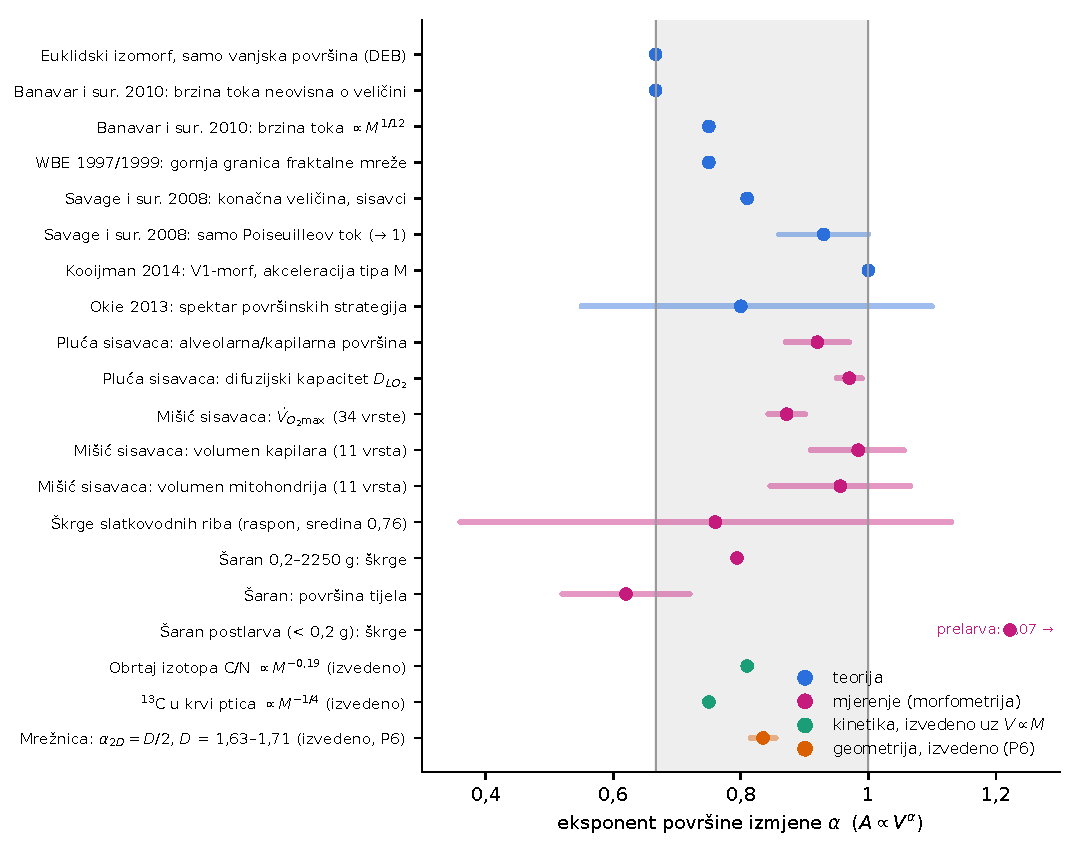
\includegraphics[width=\linewidth]{figures/fig_atlas.pdf}
\caption{Atlas eksponenata važnih za $\alpha$. Siva zona je radni raspon $2/3$–$1$. Plavo: teorijska predviđanja (T3, T8–T11). Ljubičasto: morfometrijska mjerenja s rasponom ili intervalom pouzdanosti (E1–E4). Zeleno: eksponenti izvedeni iz kinetike obrtaja uz $V\propto M$ (E6). Nagib škrga u prelarve šarana (7,07) izlazi izvan skale.}
\label{fig:atlas}
\end{figure}

\begin{kljucno}[Tri pouke iz podataka]
\begin{enumerate}[leftmargin=1.4em]
\item \textbf{Strukture za izmjenu kod sisavaca skaliraju s 0,87–0,99}, strmije od WBE granice od $3/4$ (E1, E2, E10, T8). Gustoća kapilara u mišiću gotovo ne ovisi o veličini tijela (E10). Prate \emph{vršnu} potražnju ($\dot V_{O_2\max}\propto M^{0{,}79}$–$M^{0{,}87}$), a ne bazalni metabolizam. Morfometrija je stoga gornja granica i prior za $\alpha$, a ne procjena.
\item \textbf{$\alpha$ ovisi o životnom stadiju.} Kod šarana nagib škrga pada s 7,07 na 1,22 i zatim na 0,79 (E4). Kod lososa se izmjena seli s kože na škrge (E5). Jedan $\alpha$ za cijeli život je pojednostavljenje.
\item \textbf{$\alpha$ ovisi o vrsti.} Raspon eksponenata škrga među slatkovodnim ribama je 0,36–1,13 (E3). Univerzalna vrijednost ne postoji, što je u skladu s hipotezom H6 o $\alpha$ kao svojstvu vrste ili klade.
\end{enumerate}
\end{kljucno}

\section{Što $\alpha$ radi u modelu: propozicije}\label{sec:propozicije}

\subsection{Minimalni model}

Za analizu koristimo vlastiti minimalni transportni DEB (tDEB) ovog priručnika. Model ima četiri varijable stanja: energiju u transportnom kompartimentu $E_T$, energiju u spremištu $E_E$, strukturni volumen $V$ i energiju uloženu u reprodukciju $E_R$ (slika~\ref{fig:shema}). Svi tokovi iz transporta prolaze kroz sučelje normalizirano prema jedn.~\eqref{eq:norm}:
\begin{align}
\frac{dE_T}{dt}&=\pd_A-(\beta_S+\beta_R)\,E_T\,r(V)-\beta_E\,(E_T-k_E E_E)\,r(V), \label{eq:mT}\\
\frac{dE_E}{dt}&=\beta_E\,(E_T-k_E E_E)\,r(V), \label{eq:mE}\\
\frac{dV}{dt}&=\frac{\beta_S\,E_T\,r(V)-\pM V}{\EG}, \qquad
\pd_A=\pAm\,f\,V^{2/3}\Big(\frac{V}{\Vref}\Big)^{a-2/3}. \label{eq:mV}
\end{align}
Reprodukcija prima tok $dE_R/dt=\beta_R E_T\,r(V)$.

\begin{kljucno}[Pretpostavke minimalnog modela]
\begin{enumerate}[leftmargin=1.8em,label=(\roman*)]
\item \textbf{Održavanje se plaća iz somatske grane prije rasta.} Somatski tok $\beta_S E_T\,r(V)$ najprije pokriva održavanje $\pM V$, a rast dobiva samo ostatak (jedn.~\eqref{eq:mV}). Održavanje se ne plaća izravno iz $E_T$ ni iz $E_E$.
\item \textbf{Transportni kompartiment drži malu stalnu zalihu.} U ravnoteži spremišta vrijedi $E_T=k_E E_E$ (jedn.~\eqref{eq:mE}), uz $k_E\ll1$. Brojčana vrijednost $k_E$ i procjena reda veličine iz podataka dane su u pogl.~\ref{sec:simulacije}.
\item \textbf{Smanjivanje je dopušteno pri gladovanju.} Kad somatski tok ne pokriva održavanje, $dV/dt<0$, pa se struktura troši za održavanje. Pojednostavljenje: pri smanjivanju vrijedi isti koeficijent $\EG$ kao pri rastu.
\item \textbf{Asimilacija skalira kao $V^{a}$.} Eksponent asimilacije $a$ zaseban je parametar, neovisan o $\alpha$. Za izomorfe je $a=2/3$.
\end{enumerate}
Uz to, hrana $f$ i temperatura su stalne, osim u pokusima gladovanja ($f=0$), a grana reprodukcije je ponor: nema praga zrelosti ni povratnog utjecaja na $E_T$, $E_E$ i $V$.
\end{kljucno}

\subsection{Propozicije}

\paragraph{Pretpostavka kvazi-ravnoteže.} P1–P3 pretpostavljaju da su vremenske konstante izmjene, $\big((\beta_S+\beta_R+\beta_E)\,r(V)\big)^{-1}$ za transport i $\big(\beta_E k_E\,r(V)\big)^{-1}$ za spremište (Dodatak~\ref{app:izvodi}), kratke u odnosu na vremensku skalu rasta. Za transportni kompartiment to potvrđuju podaci za čovjeka:
\begin{itemize}
\item Nakon prekida infuzije obilježivača poluvrijeme obilježenih slobodnih masnih kiselina u plazmi bilo je 3,7~$\pm$~0,1~min (11 zdravih ispitanika; Heiling, Miles i Jensen 1991) \pouzd{sažetak}.
\item Tijekom stalnog oralnog unosa masti od 175~mg\,kg$^{-1}$\,h$^{-1}$ koncentracija triglicerida u hilomikronima ustalila se na 35~$\pm$~13~mg\,dL$^{-1}$, a brzina njihova ulaska u plazmu bila je jednaka unosu (6 zdravih ispitanika; Park i sur. 2000) \pouzd{sažetak}. Uz volumen plazme od 44~mL\,kg$^{-1}$ (Haller i sur. 1992) \pouzd{sažetak} zaliha iznosi oko 15~mg\,kg$^{-1}$, pa se obrne za oko 5~min \pouzd{izvedeno}.
\end{itemize}
Vremena obrtaja od nekoliko minuta zanemariva su prema vremenskoj skali rasta; u simulacijama (pogl.~\ref{sec:simulacije}) ona iznosi $1/\dot r_B=3\EG/\pM=750$~d. Za spremište je razdvajanje mnogo slabije. U masnom tkivu čovjeka trigliceridi se obnove šest puta tijekom prosječnog desetogodišnjeg života adipocita (Arner i sur. 2011) \pouzd{sažetak}, dakle otprilike svakih 1,7 godina \pouzd{izvedeno}. Kvazi-ravnoteža spremišta zato je \emph{pretpostavka modela}, a ne posljedica podataka. Njezine posljedice kvantificiraju S4 (spremište mladih zaostaje za ravnotežom) i S5 (početni uvjeti).

\begin{propozicija}{P1 · κ-pravilo i konačna veličina ne ovise o $\alpha$}
Neka vrijedi kvazi-ravnoteža: transportni kompartiment je brz, a spremište blizu ravnoteže, $E_T\approx k_E E_E$. Tada somatski tok iznosi
\[
\pd_S=\beta_S E_T\, r(V)\approx\kappa\,\pd_A,\qquad \kappa=\frac{\beta_S}{\beta_S+\beta_R},
\]
a uz $a=2/3$ i stalnu hranu rast slijedi von Bertalanffyjevu krivulju s
\[
L_\infty=\frac{\kappa\,\pAm f}{\pM},\qquad \dot r_B=\frac{\pM}{3\EG},
\]
pri čemu nijedna od dviju veličina ne ovisi o $\alpha$. $\alpha$ utječe na rast samo kroz drugi red, tj. kroz energiju koja odlazi u punjenje spremišta.
\end{propozicija}
\textbf{Korolar P1 (κ-DEB kao poseban slučaj).} κ-DEB je poseban slučaj tDEB-a uz konstantne $\beta_S$ i $\beta_R$ u kvazi-ravnoteži. Tada se tok kroz transport dijeli u stalnom omjeru $\kappa=\beta_S/(\beta_S+\beta_R)$ između somatske grane i reprodukcije, što je upravo κ-pravilo. Ako $\beta_S$ ili $\beta_R$ ovise o stanju ili o veličini, ili ako kvazi-ravnoteža ne vrijedi, udio toka u somu više nije stalan.

\begin{propozicija}{P2 · Gustoća spremišta po strukturi}
U istoj kvazi-ravnoteži vrijedi
\[
[E_E]^{\ast}=\frac{E_E}{V}=\frac{\pAm f}{(\beta_S+\beta_R)\,k_E}\Big(\frac{V}{\Vref}\Big)^{a-\alpha}.
\]
Slaba homeostaza (gustoća neovisna o veličini) vrijedi samo za $\alpha=a$, tj. za izomorfe uz $\alpha=2/3$. Omjer gustoća između dviju veličina je $[E_E](L_1)/[E_E](L_2)=(L_1/L_2)^{3(a-\alpha)}$. Uz $a=2/3$ i $\alpha=1$ gustoća pada kao $1/L$: između $L=0{,}3$ i $L=3$~cm mijenja se deseterostruko.
\end{propozicija}
\textbf{Korolar P2 (pogrešno zadan $a$).} Nagib $\log[E_E]$ prema $\log V$ iznosi $a-\alpha$. Ako fit pretpostavlja $a=2/3$, a stvarni eksponent asimilacije je $a$, isti nagib reproducira procjena
\[
\hat\alpha\approx\alpha-(a-2/3).
\]
Za $a>2/3$ procjena je dakle pristrana prema dolje, a pristranost je jednaka pogrešci u $a$ (provjera u S6).

\textbf{P2 i ograničena homeostaza (H8).} Ako bi omjer spremišta i strukture pri stalnoj hrani trebao ostati približno stalan i kad je $\alpha=1$, P2 traži da asimilacija skalira s istim eksponentom, $a\approx\alpha$, tj. približno s volumenom. Uz izomorfnu asimilaciju ($a=2/3$) i $\alpha=1$ H8 ne vrijedi. Koja od tih kombinacija opisuje pojedinu vrstu, provjerava se mjerenjem unosa hrane prema veličini (Korak 3 i Korak 5, pogl.~\ref{sec:protokol}).

\begin{propozicija}{P3 · Vremenske konstante i gladovanje}
Sve vremenske konstante izmjene skaliraju kao $V^{1-\alpha}$. Pri gladovanju ($f=0$) spremište se prazni eksponencijalno sa specifičnom brzinom
\[
k(V)=\frac{\beta_E k_E(\beta_S+\beta_R)}{\beta_S+\beta_R+\beta_E}\; r(V)\;\propto\;V^{\alpha-1}.
\]
Nagib $\log k$ prema $\log V$ unutar vrste je dakle $\alpha-1$ i \emph{ne ovisi} o eksponentu asimilacije $a$.
\end{propozicija}

\begin{propozicija}{P4 · Identifikabilnost}
(i) Iz krivulje rasta $L(t)$ $\alpha$ praktički nije identifikabilan (P1). (ii) Gustoća spremišta prema veličini identificira razliku $a-\alpha$, pa daje $\alpha$ samo uz poznat $a$ (P2). (iii) Kinetika gladovanja prema veličini identificira $\alpha-1$ izravno (P3). Najbolji dizajn kombinira (ii) i (iii) s mjerenjem unosa hrane.
\end{propozicija}

\begin{propozicija}{P5 · Kad $\alpha$ ograničava protok}
$\alpha$ ograničava \emph{protok} energije samo ako je koncentracija u transportu ograničena regulacijom, slično kao što se regulira koncentracija glukoze u krvi. Uz $E_T/V\le[E_T]_{\max}$ najveća dostava u somu je $\propto V^{\alpha}$. Tada se $\alpha$ ponaša kao eksponent anabolizma u von Bertalanffyjevoj i GOLT logici (T15), pa uz $\alpha<1$ mreža postavlja vlastitu granicu veličine. Bez takvog ograničenja $\alpha$ mijenja samo raspodjelu i puferiranje energije, a ne ukupni protok.
\end{propozicija}

\begin{propozicija}{P6 · Fraktalna dimenzija i $\alpha$}
Neka je $D_d$ fraktalna dimenzija skupa terminalnih jedinica izmjene, a $d$ dimenzija prostora u kojem mreža leži. Tada gustoća opskrbe skalira kao $R^{D_d-d}$, pa je $\alpha=D_d/d$, a $\alpha=1$ \emph{samo} ako je $D_d=d$ (mreža ispunjava prostor). Za plošne mreže ($d=2$) dimenzije 1,3–1,7 iz H4 daju $\alpha_{2D}=0{,}65$–$0{,}85$, a ne 1. Usto, dimenzija izmjerena na slikama velikih žila ne opisuje kapilarno korito, a $\alpha$ ovisi upravo o njemu.
\end{propozicija}

\section{Rezultati simulacija}\label{sec:simulacije}

\subsection{Postavke}

Parametri su ilustrativni i ne opisuju određenu vrstu: $\pAm=100$~J\,d$^{-1}$\,cm$^{-2}$, $\pM=20$~J\,d$^{-1}$\,cm$^{-3}$, $\EG=5000$~J\,cm$^{-3}$, $\beta_S=4$, $\beta_R=1$, $\beta_E=5$~cm\,d$^{-1}$, $k_E=0{,}01$, $f=1$, $L_0=0{,}3$~cm. Odatle slijede $\kappa=0{,}8$ i $L_\infty=4$~cm, a $\Vref=(2~\text{cm})^3$. Kod je u \texttt{docs/alpha-handbook/sim/}.

\paragraph{Zašto $k_E=0{,}01$.} U ravnoteži spremišta vrijedi $E_T=k_E E_E$ (jedn.~\eqref{eq:mE}), pa je $k_E$ omjer energije u transportu i energije u spremištu. Red veličine tog omjera procjenjujemo za čovjeka, kao najbolje dokumentiranu referentnu životinju. Pretpostavljeno tijelo je muškarac od 70~kg i 1,75~m, a energijska vrijednost lipida $39$~kJ\,g$^{-1}$, kao u Koraku 3 (pogl.~\ref{sec:protokol}).
\begin{itemize}
\item \textbf{Volumen plazme:} 44~$\pm$~5~mL\,kg$^{-1}$ u 23 zdrava ispitanika (Haller i sur. 1992) \pouzd{sažetak}, dakle $\approx3{,}1$~L.
\item \textbf{Trigliceridi u plazmi:} 100~$\pm$~21~mg\,dL$^{-1}$ natašte i 237~$\pm$~40~mg\,dL$^{-1}$ tijekom stalnog unosa masti (Park i sur. 2000) \pouzd{sažetak}. To je 3,1–7,3~g, odnosno 0,12–0,28~MJ \pouzd{izvedeno}.
\item \textbf{Glukoza i slobodne masne kiseline:} uz \emph{pretpostavljene} koncentracije od 5~mmol\,L$^{-1}$ glukoze (16~kJ\,g$^{-1}$) i do 1~mmol\,L$^{-1}$ slobodnih masnih kiselina (≈270~g\,mol$^{-1}$, 39~kJ\,g$^{-1}$) sadrže još $\approx0{,}04$ i $\approx0{,}03$~MJ.
\item \textbf{Masno tkivo:} kod muškaraca normalne uhranjenosti masa masti izmjerena DXA-om iznosi 3–6~kg po m$^2$ visine (referentne vrijednosti NHANES; Kelly, Wilson i Heymsfield 2009) \pouzd{puni tekst}. Za visinu od 1,75~m to je 9–18~kg. Donja granica, 9~kg, sadrži $\approx360$~MJ \pouzd{izvedeno}.
\end{itemize}
Gornja procjena omjera je $(0{,}28+0{,}04+0{,}03)/360\approx1\times10^{-3}$, a uz trigliceride natašte $\approx5\times10^{-4}$. Uz 18~kg masti omjer se još prepolovi. Stvarni $k_E$ je dakle oko $10^{-3}$ ili manji, pa je $k_E=0{,}01$ konzervativna gornja granica s rezervom od reda veličine. Simulacije transportu pridaju veću zalihu nego što je realno, pa pretpostavka (ii) iz pogl.~\ref{sec:propozicije} kod stvarnih organizama vrijedi s još većom rezervom.

\subsection{S1 · Rast ne razlikuje $\alpha$, spremište razlikuje}

\begin{figure}[ht]
\centering
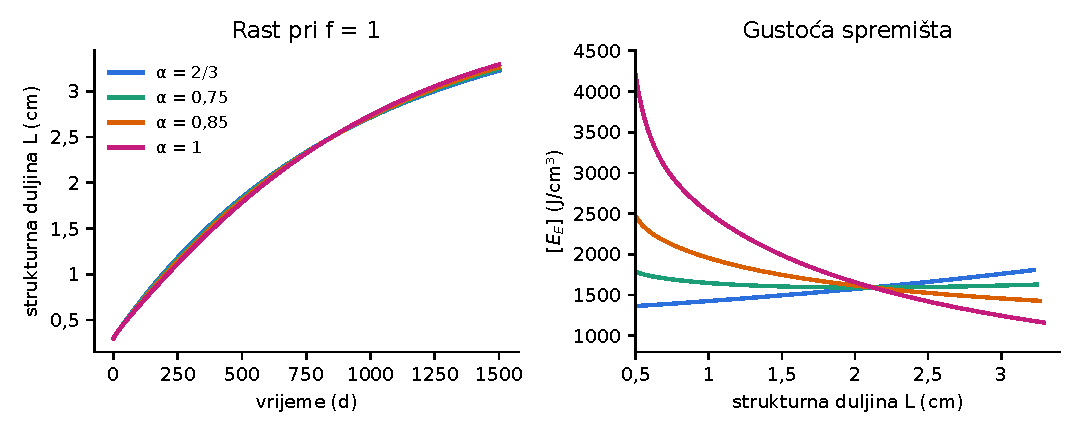
\includegraphics[width=\linewidth]{figures/fig_rast_spremiste.pdf}
\caption{Lijevo: krivulje rasta za četiri vrijednosti $\alpha$ uz iste ostale parametre. Desno: gustoća spremišta po strukturi prema strukturnoj duljini.}
\label{fig:rast}
\end{figure}

Krivulje rasta za $\alpha=2/3$ i $\alpha=1$ razlikuju se najviše oko \GrowthMaxDiff~\% (tablica~\ref{tab:rast}), a gustoća spremišta mijenja se kvalitativno. Uz $\alpha=1$ mladi su deblji od starih, a uz $\alpha=2/3$ tanji. To je numerička potvrda H7: gustoća spremišta mladih i odraslih nosi informaciju o $\alpha$, a krivulja rasta gotovo ne nosi (P1, P2).

\begin{table}[ht]
\centering\small
\caption{Rast i gustoća spremišta ($[E_E]$ u J\,cm$^{-3}$) za četiri vrijednosti $\alpha$. Nagib je $d\log[E_E]/d\log V$ za $1<L<3{,}5$~cm. „P2“ je kvazi-ravnotežno predviđanje $2/3-\alpha$. „Naivni $\alpha$“ je $2/3-\text{nagib}$, a pristranost je naivni $\alpha$ umanjen za istinski.}
\label{tab:rast}
\begin{tabular}{@{}ccccccrrrr@{}}
\toprule
$\alpha$ & $L(200)$ & $L(600)$ & $L(1500)$ & $[E_E]_{L=1}$ & $[E_E]_{L=3}$ & nagib & P2 & naivni $\alpha$ & pristranost \\
\midrule
\inputtab figures/tables/tab_growth.tex
\bottomrule
\end{tabular}
\end{table}

\subsection{S2 · Profil vjerodostojnosti}

Iz modela s $\alpha=0{,}75$ generirani su sintetski podaci: 25 mjerenja duljine s 2~\% šuma i, u drugoj varijanti, još 8 mjerenja $[E_E]$ s 10~\% šuma. Za svaki fiksirani $\alpha$ na mreži 0,50–1,00 (korak 0,025) ostali su parametri ponovno fitani ($\pAm$, $\pM$, $\beta_S$, a za drugu varijantu i $k_E$).

\begin{figure}[ht]
\centering
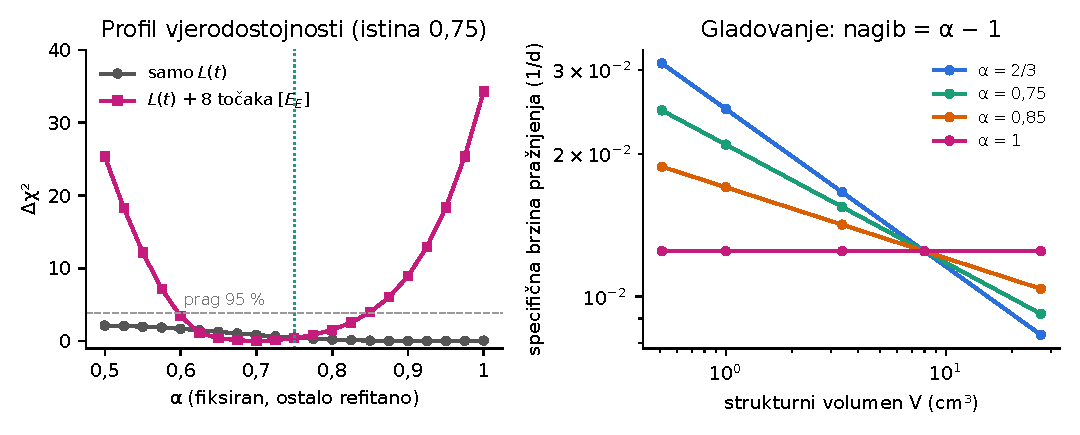
\includegraphics[width=\linewidth]{figures/fig_profil_gladovanje.pdf}
\caption{Lijevo: profil vjerodostojnosti za $\alpha$ (istinski $\alpha=0{,}75$, točkasta crta); isprekidana crta je prag 95~\% ($\Delta\chi^2=3{,}84$). Desno: specifična brzina pražnjenja spremišta pri gladovanju prema strukturnom volumenu (log–log); nagib je $\alpha-1$.}
\label{fig:profil}
\end{figure}

\begin{itemize}
\item \textbf{Samo $L(t)$:} $\Delta\chi^2\le\ProfLonlyMax$ na cijelom rasponu 0,50–1,00. Interval pouzdanosti obuhvaća cijeli raspon, pa $\alpha$ \emph{nije} identifikabilan.
\item \textbf{$L(t)$ + 8 točaka $[E_E]$:} 95~\% interval pouzdanosti seže od \CIlo{} do \CIhi{} (najbolja vrijednost na mreži \AlphaBestProf; istina 0,75). Obje granice leže unutar mreže. Profil je asimetričan: prema nižim vrijednostima raste sporije ($\Delta\chi^2=3{,}4$ pri $\alpha=0{,}60$, $25$ pri $0{,}50$), a prema višima strmo ($\Delta\chi^2\ge8{,}9$ za $\alpha\ge0{,}9$).
\end{itemize}

\subsection{S3 · Gladovanje: nagib je točno $\alpha-1$}

\begin{table}[ht]
\centering\small
\caption{Specifična brzina pražnjenja spremišta $k$ (d$^{-1}$) pri gladovanju, počevši od ravnotežnog stanja, za pet veličina ($L=0{,}8$–$3$~cm).}
\label{tab:gladovanje}
\begin{tabular}{@{}ccccc@{}}
\toprule
$\alpha$ & $k(L=1)$ & $k(L=3)$ & nagib $d\log k/d\log V$ & teorija $\alpha-1$ (P3) \\
\midrule
\inputtab figures/tables/tab_starv.tex
\bottomrule
\end{tabular}
\end{table}

Simulirani nagib poklapa se s teorijskim $\alpha-1$ (P3) unutar 0,002 za sve četiri vrijednosti $\alpha$ (tablica~\ref{tab:gladovanje}).

\subsection{S4 · Pristranost naivnog čitanja nagiba}

Tijekom rasta spremište zaostaje za ravnotežom, više kod mladih koji relativno brže rastu. Nagib gustoće spremišta zato je pomaknut prema pozitivnim vrijednostima, a naivna procjena $\alpha=2/3-\text{nagib}$ podcjenjuje istinski $\alpha$ za \NaiveBiasMin–\NaiveBiasMax{} (tablica~\ref{tab:rast}).

To je svojstvo modela, a ne numerički artefakt. Kvazi-ravnoteža spremišta (pogl.~\ref{sec:propozicije}) traži da izmjena spremišta bude brža od rasta. Vremenska konstanta izmjene spremišta, $1/k$, u simulacijama iznosi 40–120~d (tablica~\ref{tab:gladovanje}). Specifična brzina rasta volumena je približno $\dot V/V=3\dot r_B(L_\infty/L-1)$ (P1), što daje vremensku skalu od $\approx80$~d pri $L=1$~cm i $\approx750$~d pri $L=3$~cm. Kod mladih su dvije skale usporedive, pa kvazi-ravnoteža vrijedi samo približno. Kod odraslih je izmjena spremišta šest do devet puta brža od rasta, pa kvazi-ravnoteža vrijedi dobro. \textbf{Pouka:} $\alpha$ treba procjenjivati fitanjem dinamičkog modela, a ne formulom.

\subsection{S5 · Osjetljivost na početne uvjete}

\begin{figure}[ht]
\centering
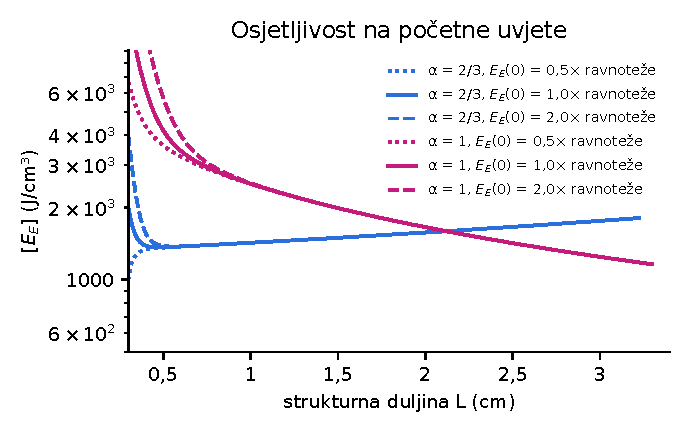
\includegraphics[width=0.66\linewidth]{figures/fig_pocetni_uvjeti.pdf}
\caption{Gustoća spremišta uz početno spremište od 0,5×, 1× i 2× ravnotežne vrijednosti, za $\alpha=2/3$ i $\alpha=1$ (početak pri $L_0=0{,}3$~cm).}
\label{fig:pu}
\end{figure}

Početno spremište postavljeno je na 0,5× ili 2× ravnotežne vrijednosti. Krivulje se ipak spajaju s referentnom (unutar 5~\%) već pri $L\approx\ICtwoThirdsLo$–$\ICtwoThirdsHi$~cm za $\alpha=2/3$, odnosno $L\approx\IConeLo$–$\IConeHi$~cm za $\alpha=1$. Razlika između $\alpha=2/3$ i $\alpha=1$ dakle nije artefakt početnih uvjeta. Kvalitativni rezultat S1 (H7) je robustan, a početni uvjeti važni su samo za najmanje jedinke.

\subsection{S6 · Monte Carlo: koji podaci otkrivaju $\alpha$}

Za svaki dizajn podataka i istinski $\alpha\in\{0{,}75;\,0{,}90\}$ generirano je \MCreps{} sintetskih skupova. Na svaki je zatim fitano šest parametara ($\pAm$, $\pM$, $\beta_S$, $k_E$, $\beta_E$, $\alpha$), s $\alpha$ ograničenim na 0,5–1,2 i dvjema početnim vrijednostima ($\alpha_0\in\{0{,}70;\,0{,}95\}$); zadržan je fit s manjim zbrojem kvadrata reziduala. Gornja granica 1,2 namjerno je iznad 1, jer se radna granica $\alpha\le1$ iz H3 pri fitanju ne smije nametnuti.
\begin{itemize}
\item Duljina $L(t)$: 25 mjerenja od 20. do 1200. dana s 2~\% šuma.
\item Spremište $[E_E]$: log-normalni šum.
\item Gladovanje: tri skupine (gladovanje počinje 200., 600. i 1200. dana, tj. pri $L\approx1$, 2 i 3~cm), spremište izmjereno 0, 10, 20 i 40 dana nakon početka, s 15~\% šuma.
\item Dizajni označeni zvjezdicom: podaci generirani s $a=0{,}72$, a fit pretpostavlja $a=2/3$ (pogrešno zadan eksponent asimilacije).
\end{itemize}

\begin{table}[ht]
\centering\small
\caption{Rezultati Monte Carlo procjene $\alpha$ (\MCreps{} ponavljanja po retku). RMSE je korijen srednje kvadratne pogreške, a zadnji stupac je udio procjena unutar $\pm0{,}05$ od istine.}
\label{tab:mc}
\begin{tabularx}{\linewidth}{@{}lXcccc r@{}}
\toprule
 & Dizajn podataka & istina & medijan $\hat\alpha$ & 10.–90. perc. & RMSE & $|\hat\alpha-\alpha|\le0{,}05$ \\
\midrule
\inputtab figures/tables/tab_mc.tex
\bottomrule
\end{tabularx}
\end{table}

\begin{figure}[ht]
\centering
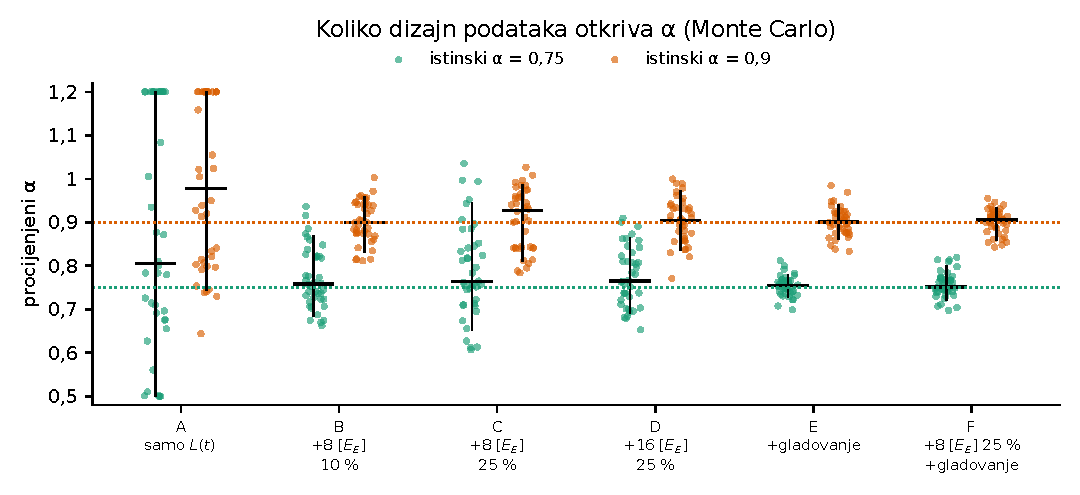
\includegraphics[width=\linewidth]{figures/fig_monte_carlo.pdf}
\caption{Procjene $\alpha$ po dizajnu podataka. Točke su pojedinačni fitovi, crne crte medijan i 10.–90. percentil, točkaste crte istinske vrijednosti. Prikazani su samo scenariji s ispravno zadanim $a$.}
\label{fig:mc}
\end{figure}

\textbf{Što pokazuje Monte Carlo:}
\begin{itemize}
\item \textbf{Samo $L(t)$ (A):} procjene se raspršuju po cijelom dopuštenom rasponu. Uz istinski $\alpha=0{,}75$ 10.–90. percentil je \MCAsevenfiveLo–\MCAsevenfiveHi, a 15–19 od \MCreps{} fitova po scenariju (37,5–47,5~\%) završi na granici raspona. RMSE je do \MCArmse. Iz samog rasta $\alpha$ nije identifikabilan; to je numerički izraz P4(i).
\item \textbf{Spremište (B–D)} smanjuje pogrešku. Uz 10~\% mjerne pogreške RMSE je do \MCBrmse{} (B), uz 25~\% do \MCCrmse{} s 8 točaka (C), odnosno do \MCDrmse{} sa 16 točaka (D). Lošija preciznost mjerenja nadoknađuje se većim brojem jedinki.
\item \textbf{Gladovanje (E) i kombinacija (F)} daju najmanju pogrešku: RMSE do \MCErmse{} (E) i \MCFrmse{} (F), uz barem 88~\% procjena unutar $\pm0{,}05$ od istine. Gladovanje je najbolji pojedinačni dizajn: nagib pražnjenja izravno daje $\alpha-1$ i ne ovisi o $a$ (P3).
\item \textbf{Pogrešno zadan $a$ pomiče $\hat\alpha$ prema dolje}, kako predviđa korolar P2: $\hat\alpha\approx\alpha-(a-2/3)=0{,}75-0{,}053\approx0{,}697$. Medijan dizajna C pada s \MCCokMed{} na \MCCmisMed, a dizajna F s \MCFokMed{} na \MCFmisMed; oba su unutar 0,012 od predviđanja. Pristranost ostaje i u dizajnu F, iako gladovanje samo po sebi ne ovisi o $a$, jer u zajedničkom fitu podaci o spremištu i rastu vuku procjenu prema pogrešnom $a$. Dizajn E s pogrešnim $a$ nije simuliran.
\item \textbf{Redoslijed za protokol:} najprije serija gladovanja u više veličina, zatim spremište po strukturi prema veličini, uz mjerenje unosa hrane prema veličini (eksponent $a$). Sam rast nikad nije dovoljan.
\end{itemize}

\begin{upozorenje}[Realnost]
Sintetski podaci su „najbolji slučaj“: nema varijabilnosti među jedinkama, a hrana i temperatura su poznate i stalne. Stvarni podaci dat će šire intervale. Rezultate treba čitati kao \emph{donju granicu} nesigurnosti i kao rangiranje dizajna, a ne kao očekivanu preciznost.
\end{upozorenje}

\begin{upozorenje}[Numerička lekcija iz ovog rada]
U prvoj verziji Monte Carla fit se zaustavljao nakon dvadesetak evaluacija, blizu početne vrijednosti $\alpha$. Uzrok je bio korak konačnih razlika za Jacobijevu matricu (zadano $\sim10^{-8}$), manji od tolerancije ODE rješavača ($10^{-7}$). Gradijent je zato bio šum, a „procjena“ je ostajala jednaka početnoj vrijednosti. Rješenje: relativni korak $10^{-3}$, više početnih vrijednosti $\alpha$ i provjera broja evaluacija. Isto vrijedi za fitanje u AmP-u (DEBtool) ili u bilo kojem drugom okruženju.
\end{upozorenje}

\section{Protokol procjene $\alpha$}\label{sec:protokol}

\subsection*{Korak 0 · Odluči što $\alpha$ opisuje}
\begin{itemize}
\item Koje sučelje: krv ↔ masno tkivo, jetra, mišić. Kod kukaca hemolimfa ↔ masno tijelo.
\item Koji supstrat: lipidi, glukoza. Kisik se tretira zasebno ($\alpha_{O_2}$) ako ima odvojenu mrežu (H5; npr. traheje kukaca, kožno disanje vodozemaca).
\item Koji stadij: za vrste s ličinkama ili metamorfozom predvidjeti barem dva $\alpha$ (E4, E5, T3).
\end{itemize}

\subsection*{Korak 1 · Klasificiraj transportnu mrežu}
Prvi filtar je tip krvotoka. U \emph{zatvorenom} krvotoku krv ostaje u zasebnim žilama ili prostorima, odvojena od međustanične tekućine, a kapilarne mreže organa poredane su usporedno. U \emph{otvorenom} krvotoku volumen krvi je veći, a protok i tlak niži, i organi se opskrbljuju serijski, pa tkiva dalje od srca dobivaju manje kisika (Monahan-Earley, Dvorak i Aird 2013). Zatvoren krvotok imaju kolutićavci (npr. gujavice) i kralježnjaci. Otvoren imaju člankonošci i većina mekušaca, npr. školjkaši; glavonošci su zatvoren krvotok razvili sekundarno (isti izvor). Granica nije uvijek oštra: i u zatvorenom krvotoku kralježnjaka sinusoidi jetre, slezene i koštane srži izravno dodiruju međustanični prostor (isti izvor).

Zatim treba utvrditi:
\begin{enumerate*}[label=(\roman*)]
\item postoji li zasebna mreža za kisik (H5); kod kukaca otvoreni krvotok ne dostavlja kisik (Monahan-Earley, Dvorak i Aird 2013), nego to rade traheje;
\item je li tijelo spljošteno, izduženo ili modularno, jer promjena oblika mijenja eksponent površine (T13, T14);
\item gradi li se mreža tijekom ontogeneze (E4, E5).
\end{enumerate*}
Rezultat određuje redak u tablici~\ref{tab:priori}.

\subsection*{Korak 2 · Postavi apriornu razdiobu}

\begin{table}[ht]
\centering\small
\caption{Radni priori za $\alpha$ po tipu mreže. Rasponi su \emph{pretpostavke}: prosudbe izvedene iz navedenih izvora, a ne mjerenja. Gornja granica $\alpha\le1$ (H3) radna je pretpostavka za izgrađenu mrežu; dok se mreža gradi, izmjereni nagibi prolazno mogu biti veći od 1 (E4).}
\label{tab:priori}
\begin{tabularx}{\linewidth}{@{}>{\raggedright\arraybackslash}p{4.3cm}>{\raggedright\arraybackslash}p{3.2cm}c>{\raggedright\arraybackslash}X@{}}
\toprule
Tip mreže & Primjeri & Prior $\alpha$ & Obrazloženje \\
\midrule
Samo difuzija, izomorfno tijelo & mali okrugli beskralježnjaci & 0,60–0,75 & euklidska geometrija (T8); $<2/3$ moguće (T11) \\
Spljošteno, izduženo ili modularno tijelo; V1-morfi & plošnjaci, trakavice, kolonije & 0,85–1,00 & V1-morf (T3); promjena oblika (T13, T14); oprez: mahovnjaci $B\propto M^{0{,}5}$ (T4) \\
Razgranat gastrovaskularni sustav & planarije, žarnjaci & 0,70–1,00 & grane se dodaju s rastom (E8); eksponent nije izmjeren \\
Otvoren krvotok (hemolimfa) & školjkaši, rakovi, \emph{Daphnia}, kukci (energija) & 0,67–1,00 & u pregledu nije nađena teorija analogna WBE-u; najveći nedostatak podataka \\
Zatvoren krvotok, nizak tlak, Poiseuilleov tok & gujavice, ličinke riba & 0,80–1,00 & T9 \\
Zatvoren pulsatilan krvotok & sisavci, ptice, odrasle ribe & 0,75–0,95 & WBE $3/4$ (T7, T8); morfometrija 0,87–0,92 (E1, E2) \\
Mreža u izgradnji (prolazno) & prelarve i postlarve riba & može biti $>1$ & E4, E5 \\
\bottomrule
\end{tabularx}
\end{table}

\subsection*{Korak 3 · Prikupi podatke}
Redoslijed slijedi korisnost za identifikaciju $\alpha$ prema P4 i Monte Carlu (S6, tablica~\ref{tab:mc}). Krivulja rasta korisna je za ostale parametre, ali sama nikad nije dovoljna.
\begin{enumerate}[leftmargin=1.6em]
\item \textbf{Serija gladovanja prema veličini.} Barem tri veličinske klase, barem četiri vremenske točke po klasi i ista temperatura. Mjeriti zalihe (lipide, glikogen), a ne samo masu tijela. Nagib $\log k$ prema $\log V$ daje $\alpha-1$ i ne ovisi o eksponentu asimilacije $a$ (P3). U S6 je to najbolji pojedinačni dizajn (E, RMSE do \MCErmse).
\item \textbf{Spremište po strukturi prema veličini}, pri poznatoj hrani i temperaturi. Gustoća spremišta skalira kao $V^{a-\alpha}$ (P2), pa daje $\alpha$ samo uz poznat $a$. \emph{Pretvorba:} literatura obično navodi lipide po cijelom tijelu, a model spremište po strukturi (H7). Ako je $\varphi$ maseni udio lipida (na istoj osnovici, mokroj ili suhoj), gustoća spremišta po strukturi je $[E_E]\propto\varphi/(1-\varphi)$, a ne $\varphi$. Za energiju se može uzeti uobičajena približna vrijednost topline izgaranja lipida, $\approx39$~kJ\,g$^{-1}$. Ta konstanta ne utječe na nagib $\log[E_E]$ prema $\log V$, pa ni na $\hat\alpha$; utječe samo na apsolutne vrijednosti parametara.
\item \textbf{Unos hrane prema veličini} (eksponent $a$). Bez njega gustoća spremišta daje samo razliku $a-\alpha$ (P2), a pogrešno zadan $a$ pristrano pomiče $\hat\alpha$ (S6, dizajni sa zvjezdicom).
\item \textbf{Morfometrija} (stereologija površine izmjene po jedinici volumena, $S_V\propto V^{\alpha-1}$) služi kao prior ili gornja granica (E1, E2, T15).
\item \textbf{Obrtaj obilježivača} (stabilni izotopi, klirens lipida iz plazme) služi samo kao provjera, jer miješa obrtaj proteina i razrjeđenje rastom (E6).
\item \textbf{AmP:} postojeći parametri i $s_M$ (T3) za kontekst i kao početne vrijednosti.
\end{enumerate}

\begin{kljucno}[Najmanji dizajni prema Monte Carlu (S6)]
Svi dizajni u S6 uključuju i krivulju rasta: 25 mjerenja duljine s 2~\% šuma. Podaci su idealizirani (bez varijabilnosti među jedinkama, uz poznatu i stalnu hranu i temperaturu), pa su brojke donja granica nesigurnosti i služe za rangiranje dizajna.
\begin{itemize}[leftmargin=1.4em]
\item \textbf{Preporučeno, gladovanje (E):} 3 veličinske klase ($L\approx1$, 2 i 3~cm, tj. trostruki raspon duljine) × 4 vremenske točke (0, 10, 20 i 40 dana nakon uklanjanja hrane), s 15~\% mjerne pogreške zaliha. RMSE je do \MCErmse, a otprilike 9 od 10 procjena leži unutar $\pm0{,}05$ od istine. Do zadnje točke spremište u S6 padne na približno 45–70~\% početne vrijednosti; za drugu vrstu vremenske točke treba birati tako da pokriju sličan pad.
\item \textbf{Bez gladovanja, samo spremište (B, D):} 8 veličina uz $\le10$~\% mjerne pogreške (RMSE do \MCBrmse) ili 16 veličina uz $\sim25$~\% (RMSE do \MCDrmse). Uz 8 veličina i 25~\% pogreške (C) RMSE raste do \MCCrmse. Točke spremišta u S6 pokrivaju $L\approx0{,}6$–3~cm, tj. barem četverostruki raspon duljine.
\item \textbf{Kombinacija (F):} 8 veličina spremišta (25~\%) i gladovanje kao u E. RMSE do \MCFrmse.
\item \textbf{Nedovoljno, samo rast (A):} procjene se raspršuju po cijelom dopuštenom rasponu (10.–90.~percentil \MCAsevenfiveLo–\MCAsevenfiveHi{} za istinski $\alpha=0{,}75$), 38–47~\% fitova završi na granici raspona, a RMSE je do \MCArmse.
\item \textbf{Uz svaki dizajn izmjeriti unos prema veličini.} Ako je istinski $a=0{,}72$, a fit pretpostavlja $2/3$, $\hat\alpha$ je pristran naniže: medijan dizajna C pada s \MCCokMed{} na \MCCmisMed, a dizajna F s \MCFokMed{} na \MCFmisMed{} (istina 0,75). To se slaže s P2, prema kojoj je $\hat\alpha\approx\alpha-(a-2/3)$. Ni gladovanje ne uklanja pristranost kad su u fitu i spremište i rast (F). Za dizajn E pogrešno zadan $a$ nije testiran.
\end{itemize}
\end{kljucno}

Vrste treba birati prema dostupnosti \emph{ovih} podataka, prije svega gladovanja i spremišta po veličinama. Unos u AmP-u sam po sebi nije dovoljan razlog za odabir, jer se iz krivulje rasta $\alpha$ ne može procijeniti (P4, S6). Idealne su vremenske serije veličine, mase, dobi i lipida, po mogućnosti odvojeno za krv i tijelo.

\subsection*{Korak 4 · Fitaj}
\begin{enumerate}[leftmargin=1.6em]
\item Parametriziraj prema jedn.~\eqref{eq:norm} s $\Vref=V_b$.
\item Fitaj sve podatke zajedno. Za spremište i gladovanje koristi logaritamske reziduale, s težinama iz mjerne pogreške.
\item Koristi barem dvije početne vrijednosti $\alpha$ (npr. 0,70 i 0,95). Korak konačnih razlika mora biti veći od tolerancije rješavača (u S6 relativni korak $10^{-3}$ uz toleranciju $10^{-7}$). Provjeri da se fit nije zaustavio na početnoj vrijednosti.
\item Provjeri je li $\hat\alpha$ završio na granici dopuštenog raspona. To je znak da $\alpha$ nije identificiran: u S6 se to dogodilo u 38–47~\% fitova samo na rast (A), a ni u jednom fitu s gladovanjem (E, F).
\item Izračunaj profil vjerodostojnosti za $\alpha$ na mreži 0,55–1,10 s korakom 0,025 i navedi 95~\% interval pouzdanosti ($\Delta\chi^2=3{,}84$).
\item Ako interval obuhvaća cijeli raspon $[2/3,1]$, $\alpha$ \emph{nije} procijenjen. Navedi prior i to jasno napiši.
\item Bayesovska alternativa: prior iz tablice~\ref{tab:priori} i aposteriorna razdioba za $\alpha$.
\end{enumerate}

\subsection*{Korak 5 · Provjeri}
\begin{itemize}
\item \textbf{Predikcija izvan uzorka:} model fitan na rast i spremište treba predvidjeti krivulju gladovanja, ili obrnuto.
\item \textbf{Osjetljivost:} na $a$ (S6), na početne uvjete (S5), na $\Vref$ i na temperaturu.
\item \textbf{Usporedba s morfometrijom:} ako je $\hat\alpha$ znatno iznad morfometrijskog eksponenta, to treba objasniti, npr. gustoćom transportera, jer je „površina“ generalizirana (H2).
\item \textbf{Biološka prihvatljivost (H8):} je li promjena gustoće spremišta s veličinom koju model predviđa (P2) prihvatljiva za tu vrstu?
\end{itemize}

\subsection*{Korak 6 · Filogenetski test}
Za svaku vrstu navedi $\hat\alpha$ s intervalom pouzdanosti. Zatim:
\begin{enumerate*}[label=(\roman*)]
\item usporedi tipove mreža filogenetskom regresijom (PGLS) s težinama iz intervala;
\item procijeni filogenetski signal (Pagelov $\lambda$, Pagel 1999; Blombergov $K$, Blomberg, Garland i Ives 2003) i time testiraj H6;
\item testiraj H9, tj. poklapa li se $\alpha$ s determiniranim ili indeterminiranim rastom.
\end{enumerate*}

\textbf{Koliko vrsta.} U simulacijama Blomberga, Garlanda i Ivesa (2003) randomizacijski test filogenetskog signala ima ispravnu stopu pogreške tipa I (uz razinu značajnosti 0,05) i dobru snagu (0,8) za skupove od 20 ili više vrsta. Iz toga slijedi da je približno 20 vrsta s procijenjenim $\alpha$ donja granica za smislen test H6, a ne luksuz.

\begin{kljucno}[Kontrolna lista prije objave vrijednosti $\alpha$]
\begin{itemize}[label=$\square$,leftmargin=1.6em]
\item Jasno je koje sučelje i koji supstrat $\alpha$ opisuje (energija ili kisik).
\item Uz rast postoje podaci o gladovanju ili o spremištu po veličinama; rast sam nije dovoljan.
\item Spremište je izraženo po \emph{strukturi}, ne po ukupnoj masi.
\item Eksponent asimilacije $a$ je izmjeren ili je navedena pretpostavka.
\item Podaci su intraspecifični i ontogenetski, pri poznatoj hrani i temperaturi.
\item Fit je pokrenut iz barem dviju početnih vrijednosti $\alpha$, nije zapeo na početnoj vrijednosti i nije završio na granici raspona.
\item Naveden je profil vjerodostojnosti i 95~\% interval pouzdanosti.
\item Provjerena je osjetljivost na $a$ i na početne uvjete.
\item Navedeno je je li $\alpha$ ovisan o stadiju.
\end{itemize}
\end{kljucno}

\section{Česte zamke}\label{sec:zamke}

\begin{enumerate}[leftmargin=1.6em]
\item \textbf{$\alpha=b$.} Metabolički eksponent miješa tokove koji skaliraju s $V^{2/3}$, $V$ i $V^{\alpha}$ te ovisi o udjelu rezerve u masi (T1, T2). Isti raspon $[2/3,1]$ za $b$ (T12) i za $\alpha$ posljedica je istog miješanja površinskih i volumnih procesa, a ne dokaz da su jednaki.
\item \textbf{Masa umjesto strukture.} MTE izražava skaliranje prema ukupnoj masi $M$ (T7–T9), a DEB razlikuje strukturu i rezervu i skalira prema strukturi (T1, T2). Ako gustoća spremišta ovisi o veličini (P2), eksponenti po masi i po strukturi se razlikuju. Isto vrijedi za udio lipida: udio po ukupnoj masi $\varphi$ treba pretvoriti u $\varphi/(1-\varphi)$ (pogl.~\ref{sec:protokol}, Korak 3).
\item \textbf{Interspecifično umjesto intraspecifičnog.} Interspecifični $3/4$ uključuje promjenu parametara među vrstama (T2). $\alpha$ je ontogenetski eksponent.
\item \textbf{Kisik i energija kao jedna mreža.} Traheje kukaca i kožno disanje vodozemaca odvajaju kisik od energije (H5).
\item \textbf{Morfometrija kao procjena.} Strukture prate vršnu potražnju i skaliraju strmije od bazalnog metabolizma (E1, E2, T15). Morfometrija daje prior, ne $\alpha$.
\item \textbf{Fraktalna dimenzija sa slika.} Dimenzija manja od dimenzije prostora znači da mreža \emph{ne} ispunjava prostor, pa je $\alpha<1$ (H4, P6).
\item \textbf{Nagib bez dinamike.} Spremište zaostaje za rastom, a naivna procjena pristrana je za \NaiveBiasMin–\NaiveBiasMax{} (S4).
\item \textbf{Jedan $\alpha$ za cijeli život.} Kod riba se mreža izmjene mijenja s kože na škrge (E4, E5).
\item \textbf{Fitanje samo na rast.} $\alpha$ tada nije identifikabilan (P1, S2, S6).
\item \textbf{Pretpostavljeni umjesto izmjerenog $a$.} Ako je istinski $a$ veći od pretpostavljenog $2/3$, $\hat\alpha$ je pristran naniže za približno $a-2/3$ (P2), i to i uz podatke o gladovanju kad su u fitu i spremište i rast (S6).
\item \textbf{$\beta$ bez normalizacije.} Jedinice $\beta$ ovise o $\alpha$, pa se $\beta$ ne mogu uspoređivati među vrstama s različitim $\alpha$ (pogl.~\ref{sec:definicija}). Koristiti jedn.~\eqref{eq:norm}.
\item \textbf{Parametri bez dokumentiranog izvora.} Ilustrativne vrijednosti, poput onih u pogl.~\ref{sec:simulacije}, lako se prenesu u analizu kao da su procjene za stvarnu vrstu. Svaki parametar treba imati dokumentiran izvor: mjerenje, literaturu s navedenim podacima ili fit s navedenim podacima i postupkom.
\end{enumerate}

\section{Kandidatske vrste}\label{sec:vrste}

\providecommand{\vrstaVE}[1]{\leavevmode{\sffamily\bfseries\color{akcent}VE#1}}

Tablica~\ref{tab:vrste} predlaže vrste za prvu procjenu $\alpha$ prema protokolu iz pogl.~\ref{sec:protokol}. Vrste su birane prema trima kriterijima:
\begin{enumerate}[leftmargin=1.6em]
\item \textbf{Pokrivenost tipova mreže.} Vrste zajedno trebaju pokriti tipove transportne mreže iz tablice~\ref{tab:priori}, jer se H3 i H6 mogu testirati tek usporedbom tipova.
\item \textbf{Postojeći podaci.} Prednost imaju vrste za koje su već objavljeni podaci o spremištu prema veličini, o unosu hrane prema veličini (eksponent $a$) i o gladovanju u više veličina. Upravo ti podaci identificiraju $\alpha$; krivulja rasta to ne može (P2–P4, S6).
\item \textbf{Broj vrsta.} Za razvoj i provjeru metode predlažemo najmanje pet vrsta s različitim tipovima mreže. Za filogenetski test (Korak~6) treba približno 20 vrsta: randomizacijski test filogenetskog signala ima dobru snagu (0,8) na simuliranim skupovima s 20 ili više vrsta (Blomberg, Garland i Ives 2003).
\end{enumerate}

Za svaku vrstu tablica navodi tip mreže, radni prior iz tablice~\ref{tab:priori}, objavljene podatke s brojkama (oznake VE1–VE14) i što još treba izmjeriti. Navedeno je i ima li vrsta unos u zbirci Add-my-Pet (AmP; Marques i sur. 2018), prema popisu vrsta na \url{https://www.bio.vu.nl/thb/deb/deblab/add_my_pet/species_list.html} (stanje 3.~11.~2026.); u zagradi je tip modela. Parametri iz AmP-a služe kao početne vrijednosti i ne zamjenjuju mjerenja iz Koraka~3. Tip rasta (H9) naveden je samo ondje gdje ga izvor dokumentira.

Najpotpunije podatke imaju planarije i komarča: za obje su objavljeni unos, spremište i gladovanje prema veličini (VE1–VE3, VE5–VE7). Kod ostalih vrsta nedostaje barem jedan od tih triju tipova podataka. Pokrivenost ima dvije praznine. Za tip „samo difuzija, izomorfno tijelo“ nismo našli vrstu s objavljenim unutarvrsnim podacima o spremištu ili gladovanju prema veličini. Gujavice (zatvoren krvotok niskog tlaka) imaju unose u AmP-u (\emph{Lumbricus terrestris}, \emph{Eisenia fetida}, oba \texttt{std}), ali takve podatke nismo našli, pa nisu u tablici. Taj tip mreže djelomično pokrivaju ličinke riba.

{\footnotesize
\setlength{\tabcolsep}{4pt}
\begin{longtable}{@{}>{\raggedright\arraybackslash}p{2.2cm}>{\raggedright\arraybackslash}p{2.4cm}>{\raggedright\arraybackslash}p{1.6cm}>{\raggedright\arraybackslash}p{6.0cm}>{\raggedright\arraybackslash}p{2.75cm}@{}}
\caption{Kandidatske vrste za procjenu $\alpha$. VE označava objavljeni podatak uz ovu tablicu; E, T i H upućuju na izjave iz poglavlja~\ref{sec:definicija}–\ref{sec:empirija}.}\label{tab:vrste}\\
\toprule
Vrsta / skupina & Mreža & Prior $\alpha$ & Što je poznato & Što treba izmjeriti \\
\midrule
\endfirsthead
\toprule
Vrsta / skupina & Mreža & Prior $\alpha$ & Što je poznato & Što treba izmjeriti \\
\midrule
\endhead
\bottomrule
\endfoot
Planarije (\emph{Schmidtea mediterranea})
& bez krvotoka; razgranato crijevo i difuzija
& 0,70–1,00
& E7, E8.
\par \vrstaVE{1} Rast je reverzibilan: duljina se mijenja između $\approx0{,}5$ i $\approx20$~mm, a gladne jedinke se smanjuju gubitkom stanica. Metabolizam $\propto M^{0{,}75\pm0{,}01}$ (vlažna masa), broj stanica $\propto M^{0{,}74\pm0{,}01}$ (suha masa).
\par \vrstaVE{2} Spremište: triacilgliceroli po stanici 88 puta, a glikogen 8 puta veći kod jedinki od 16~mm nego od 4~mm. Lipidne kapljice su uglavnom u crijevnom epitelu. Energija po stanici $\propto N^{0{,}38\pm0{,}03}$ ($N$ broj stanica).
\par \vrstaVE{3} Volumen obroka (ad libitum) proporcionalan je broju stanica (eksponent po stanici $0{,}00\pm0{,}03$). Brzina smanjivanja pri gladovanju (\% površine na dan) pada s veličinom, kao i brzina rasta, i jednaka je nakon 1–4, 4–7 i 7–10 tjedana gladovanja. (Thommen i sur. 2019) \pouzd{puni tekst}
\par AmP: samo srodna \emph{S. polychroa} (\texttt{abj}).
& lipidi po strukturi (broj stanica kao mjera strukture) prema veličini; pražnjenje lipida, a ne samo površine, pri gladovanju u $\ge3$ veličine; brzina unosa, a ne jedan obrok \\
\addlinespace
Trakavica (\emph{Hymenolepis diminuta})
& bez krvotoka; hrana se upija kroz površinu tijela (tegument)
& 0,85–1,00
& \vrstaVE{4} In vitro, u 6~mM glukoze: crv od 5~mg suhe mase upija 80, a crv od 60~mg 35~$\mu$mol glukoze po g suhe mase u 5~min. Autor pad pripisuje manjem omjeru površine i mase. Upijanje po masi pada i s brojem crva u domaćinu: 111, 88 i 77~$\mu$mol\,g$^{-1}$ za 1, 7–8 i 45–50 crva. (Henderson 1977) \pouzd{sažetak}
\par Iz prvih dviju točaka ukupno upijanje $\propto M^{0{,}67}$ \pouzd{izvedeno}, ispod priora za spljošteno tijelo; dob i veličina tu nisu razdvojene.
\par AmP: nema trakavica.
& spremište (glikogen) po strukturi prema veličini; gladovanje domaćina kao pokus gladovanja; razdvojiti dob, veličinu i gustoću crva \\
\addlinespace
Šaran (\emph{Cyprinus carpio}), losos (\emph{Oncorhynchus tshawytscha})
& koža, zatim škrge; zatvoren krvotok u izgradnji
& stadijski: $>1$ moguće u ličinki, 0,75–0,95 kasnije
& E4: nagib površine škrga je 7,07 u prelarve, 1,22 u postlarve (do 0,2~g) i 0,79 između 0,2 i 2250~g. E5: pri izlijeganju koža čini $\approx96$~\% površine izmjene, a škrge je prestižu pri 2,5–4~g.
\par AmP: obje vrste (\texttt{abj}).
& $\alpha$ po stadiju; spremište, unos i gladovanje ličinki i mlađi u više veličina \\
\addlinespace
Komarča (\emph{Sparus aurata})
& zatvoren pulsatilan krvotok
& 0,75–0,95
& \vrstaVE{5} Sastav tijela izmjeren je u 44 skupine riba od 1 do 470~g na komercijalnoj hrani ($W$ je masa u g). Lipidi (mg po g vlažne mase) $=43{,}3\,W^{0{,}243}$, tj. od 43 do 186~mg/g kod riba od $\approx400$~g. Proteini su stalni (176~mg/g), a energija raste od 4,7 do 11,0~kJ/g.
\par \vrstaVE{6} Unos hrane $=0{,}029\,W^{0{,}598}e^{0{,}057T}$~g po ribi na dan; prirast $=0{,}024\,W^{0{,}514}e^{0{,}060T}$~g na dan ($T$ u~°C; 1–450~g, 20–28~°C).
\par \vrstaVE{7} Gladovanje do 30 dana: gubitak energije $41{,}5\,W_{\mathrm{kg}}^{0{,}82}$~kJ po ribi na dan i gubitak proteina $0{,}40\,W_{\mathrm{kg}}^{0{,}70}$~g na dan ($W_{\mathrm{kg}}$ u kg). (Lupatsch, Kissil i Sklan 2003) \pouzd{puni tekst}
\par AmP: da (\texttt{abj}).
& lipidi po strukturi (ne po vlažnoj masi) pri poznatom obroku; lipidi, a ne samo ukupna energija, tijekom gladovanja u $\ge3$ veličine \\
\addlinespace
\emph{Daphnia magna}
& otvoren krvotok (hemolimfa)
& 0,67–1,00
& \vrstaVE{8} Kod \emph{D. magna} i \emph{D. galeata mendotae} količina triacilglicerola korelira s ukupnom biomasom, neovisno o duljini tijela. Biomasa odrasle jedinke tijekom jednog razdoblja između presvlačenja naraste 2–3 puta, a triacilgliceroli čine 16~\% tog prirasta. Pred kraj tog razdoblja spremište prelazi u jajnike. Mladi s mnogo majčinih lipida preživljavaju gladovanje dvostruko dulje od mladih slične mase s malo lipida. (Tessier i sur. 1983) \pouzd{sažetak}
\par \vrstaVE{9} Međuvrsno, za zooplankton pri 20~°C: vrijeme preživljavanja gladovanja $t=2{,}95\,w^{0{,}25}$~dana ($w$ u $\mu$g suhe mase). Izraz je uspoređen s podacima za 25 vrsta i s novim podacima za \emph{D. magna}; starije jedinke preživljavaju kraće od predviđenog. (Threlkeld 1976) \pouzd{sažetak}
\par AmP: da (\texttt{std}).
& lipidi po strukturi prema veličini u istoj fazi presvlačenja; gladovanje u $\ge3$ veličine (lipidi, ne preživljavanje); odvojiti spremište od jajnika \\
\addlinespace
Dagnja (\emph{Mytilus edulis})
& otvoren krvotok
& 0,67–1,00
& \vrstaVE{10} Najveća brzina filtracije $F=6{,}773\,W^{0{,}678}$~l/h ($W$ suha masa mekog tkiva u g) i $F\propto L^{2{,}088}$ ($L$ duljina ljušture). Indeks kondicije $W/L^3$ razlikuje se među populacijama i tijekom godine. (Riisgård, Larsen i Pleissner 2014) \pouzd{sažetak}
\par \vrstaVE{11} Uz hranu ispod potrebe za održavanje potrošnja kisika za 35–40 dana padne na standardnu razinu (Bayne 1973). Pri temperaturnom i prehrambenom stresu gube se ugljikohidrati i proteini, relativno više iz plašta, u kojem je gonada, nego iz ostalih tkiva (Gabbott i Bayne 1973). \pouzd{sažetak}
\par AmP: \emph{M. edulis} i \emph{M. galloprovincialis} (\texttt{abj}).
& glikogen i lipidi po strukturi prema veličini, izvan razdoblja zrenja gonade; gladovanje u $\ge3$ veličine; odvojiti spremište od gonade \\
\addlinespace
Kukci (\emph{Manduca sexta})
& otvoren krvotok: hemolimfa za energiju, traheje za kisik (H5)
& $\alpha_E$: 0,67–1,00; $\alpha_{O_2}$ zasebno
& T6: unos hrane skalira ontogenetski s eksponentom 0,70.
\par \vrstaVE{12} Velike traheje određene su pri presvlačenju i ne rastu do idućega, a ličinka unutar jednog stupnja naraste do 10 puta u masi (Callier i Nijhout 2012). U zadnjem stupnju ličinke trahejni sustav ipak znatno raste u masi i volumenu (Helm i Davidowitz 2013). \pouzd{sažetak}
\par \vrstaVE{13} Udio masti raste kroz sve stadije, uključujući lutanje i metamorfozu, na svim ispitanim umjetnim hranama; jedinke na hrani s manje saharoze znatno su mršavije. (Ojeda-Avila, Woods i Raguso 2003) \pouzd{sažetak}
\par AmP: da (\texttt{hex}).
& lipidi masnog tijela po strukturi prema veličini \emph{unutar} stupnja; gladovanje unutar stupnja u više veličina; $\alpha_E$ i $\alpha_{O_2}$ odvojeno \\
\addlinespace
Miš (\emph{Mus musculus})
& zatvoren pulsatilan krvotok
& 0,75–0,95
& E1, E2, E10 (međuvrsno, sisavci): površina pluća $\propto M^{0{,}92}$; volumen kapilara lokomotornih mišića $\propto M^{0{,}98}$, uz gotovo stalnu gustoću kapilara.
\par \vrstaVE{14} Četrdeset inbred sojeva u dobi od $\approx16$ tjedana: srednja masa soja 11,4–39,3~g, udio masti 16–39~\%. Teži sojevi su masniji ($r=0{,}57$), no neki laki sojevi također su masni (SPRET/EiJ: 15,7~g i 26~\% masti). (Reed, Bachmanov i Tordoff 2007) \pouzd{sažetak}
\par AmP: da (\texttt{stx}).
& masno tkivo po strukturi (npr. bezmasnoj masi) prema veličini unutar jednog soja, spola i dobi; gladovanje u više veličina \\
\addlinespace
Mahovnjaci (Bryozoa)
& modularne kolonije
& 0,85–1,00 (oprez: T4)
& T4: u kolonijama s pokusno smanjenom i netaknutom veličinom $B\propto M^{0{,}5}$; DEB model alokacije objašnjava eksponent i apsolutnu vrijednost $B$.
\par AmP: četiri vrste, npr. \emph{Flustra foliacea} (\texttt{std}).
& spremište po zooidu prema veličini kolonije; gladovanje kolonija različite veličine \\
\end{longtable}
}

\section{Otvorena pitanja}\label{sec:otvoreno}

\begin{enumerate}[leftmargin=1.6em]
\item \textbf{Koja varijanta modela daje H9?} Hipoteza H9 povezuje $\alpha\neq1$ s indeterminiranim rastom. Minimalni model to ne reproducira: $L_\infty$ ne ovisi o $\alpha$ (P1), a uz ograničen protok (P5) upravo $\alpha<1$ postavlja granicu veličine, dakle suprotno od H9. Ne pomaže ni varijanta u kojoj asimilacija prolazi kroz isto sučelje ($a=\alpha$): uz $a=1$ jedn.~\eqref{eq:mV} u kvazi-ravnoteži daje $dV/dt\propto V$, tj. rast bez asimptote kao kod V1-morfa (T3). Indeterminirani rast tada bi pratio $\alpha=1$, a ne $\alpha\neq1$. Otvoreno je koja pretpostavka može dati H9, npr. rast izvan kvazi-ravnoteže ili drukčije pravilo održavanja ili reprodukcije.
\item \textbf{Homeostaza (H8) i P2.} Prema P2 gustoća spremišta skalira kao $V^{a-\alpha}$. Uz $a=2/3$ i $\alpha=1$ mijenja se deseterostruko između $L=0{,}3$ i $3$~cm, što je teško uskladiti s H8. H8 je zadovoljena samo uz $a\approx\alpha$ (Dodatak~\ref{app:izvodi}). Otvoreno je prolazi li asimilacija doista kroz isto sučelje kao izmjena sa spremištem ili su $a$ i $\alpha$ povezani na drugi način. Odgovor daju mjerenja unosa i spremišta prema veličini (pogl.~\ref{sec:protokol}, Korak 3).
\item \textbf{Regulator koncentracije u transportu (P5).} Uvodi li se, $\alpha$ postaje ograničenje protoka i počinje utjecati na rast.
\item \textbf{κ-DEB kao poseban slučaj tDEB-a.} Uz konstantne $\beta_S$ i $\beta_R$ P1 u kvazi-ravnoteži daje κ-pravilo s $\kappa=\beta_S/(\beta_S+\beta_R)$. Formalni izvod izvan kvazi-ravnoteže ostaje otvoren.
\item \textbf{Dva $\alpha$} (energija i kisik, H5) i njihovo sprezanje u jednadžbama modela.
\item \textbf{$\alpha$ ovisan o stadiju}, tj. veza s akceleracijom tipa M (T3).
\item \textbf{Troškovi transporta.} Minimalni model ne sadrži trošak rada transportne mreže. Otvoreno je koliki je taj trošak, ovisi li o $\alpha$ i koliko pridonosi respiraciji.
\item \textbf{Kvazi-ravnoteža kod mladih.} P1–P3 pretpostavljaju da su $E_T$ i $E_E$ u kvazi-ravnoteži. To je ograda modela: kod mladih, koji relativno brže rastu, spremište zaostaje za ravnotežom (S4), a početni uvjeti važni su za najmanje jedinke (S5). Otvoreno je kako tu ogradu ugraditi u procjenu za vrste s brzim ranim rastom.
\item \textbf{Otvoreni krvotoci.} U pregledu za ovaj priručnik nije nađena teorija analogna WBE-u za otvorene krvotoke, a to je najveća praznina (tablica~\ref{tab:priori}).
\item \textbf{Prazan prostor u literaturi.} Pregledom nije nađen rad koji DEB spaja s razgranatom opskrbnom mrežom ili tretira eksponent površine kao slobodan parametar, osim kroz funkciju korekcije oblika i V1-morfe (T3). To je prilika za objavu.
\end{enumerate}

\section*{Literatura}
\addcontentsline{toc}{section}{Literatura}
\begin{small}\raggedright
\begin{enumerate}[label={},leftmargin=1.2em,itemindent=-1.2em,itemsep=0.15em]
\item Arner P, Bernard S, Salehpour M, Possnert G, Liebl J, Steier P, Buchholz BA, Eriksson M, Arner E, Hauner H, Skurk T, Rydén M, Frayn KN, Spalding KL (2011). Dynamics of human adipose lipid turnover in health and metabolic disease. \emph{Nature} 478(7367):110–113. \href{https://doi.org/10.1038/nature10426}{doi:10.1038/nature10426}
\item Banavar JR, Moses ME, Brown JH, Damuth J, Rinaldo A, Sibly RM, Maritan A (2010). A general basis for quarter-power scaling in animals. \emph{PNAS} 107(36):15816–15820. \href{https://doi.org/10.1073/pnas.1009974107}{doi:10.1073/pnas.1009974107}
\item Bayne BL (1973). Physiological changes in \emph{Mytilus edulis} L. induced by temperature and nutritive stress. \emph{Journal of the Marine Biological Association of the United Kingdom} 53(1):39–58. \href{https://doi.org/10.1017/S0025315400056629}{doi:10.1017/S0025315400056629}
\item Blomberg SP, Garland T, Ives AR (2003). Testing for phylogenetic signal in comparative data: behavioral traits are more labile. \emph{Evolution} 57(4):717–745. \href{https://doi.org/10.1111/j.0014-3820.2003.tb00285.x}{doi:10.1111/j.0014-3820.2003.tb00285.x}
\item Callier V, Nijhout HF (2012). Supply-side constraints are insufficient to explain the ontogenetic scaling of metabolic rate in the tobacco hornworm, \emph{Manduca sexta}. \emph{PLoS ONE} 7(9):e45455. \href{https://doi.org/10.1371/journal.pone.0045455}{doi:10.1371/journal.pone.0045455}
\item Carleton SA, Martínez del Rio C (2005). The effect of cold-induced increased metabolic rate on the rate of $^{13}$C and $^{15}$N incorporation in house sparrows (\emph{Passer domesticus}). \emph{Oecologia} 144(2):226–232. \href{https://doi.org/10.1007/s00442-005-0066-8}{doi:10.1007/s00442-005-0066-8}
\item Forsthoefel DJ, Park AE, Newmark PA (2011). Stem cell-based growth, regeneration, and remodeling of the planarian intestine. \emph{Developmental Biology} 356(2):445–459. \href{https://doi.org/10.1016/j.ydbio.2011.05.669}{doi:10.1016/j.ydbio.2011.05.669}
\item Gabbott PA, Bayne BL (1973). Biochemical effects of temperature and nutritive stress on \emph{Mytilus edulis} L. \emph{Journal of the Marine Biological Association of the United Kingdom} 53(2):269–286. \href{https://doi.org/10.1017/S0025315400022268}{doi:10.1017/S0025315400022268}
\item Gazit Y, Berk DA, Leunig M, Baxter LT, Jain RK (1995). Scale-invariant behavior and vascular network formation in normal and tumor tissue. \emph{Physical Review Letters} 75(12):2428–2431. \href{https://doi.org/10.1103/PhysRevLett.75.2428}{doi:10.1103/PhysRevLett.75.2428}
\item Gehr P, Mwangi DK, Ammann A, Maloiy GMO, Taylor CR, Weibel ER (1981). Design of the mammalian respiratory system. V. Scaling morphometric pulmonary diffusing capacity to body mass: wild and domestic mammals. \emph{Respiration Physiology} 44(1):61–86. \href{https://doi.org/10.1016/0034-5687(81)90077-3}{doi:10.1016/0034-5687(81)90077-3}
\item Glazier DS (2010). A unifying explanation for diverse metabolic scaling in animals and plants. \emph{Biological Reviews} 85(1):111–138. \href{https://doi.org/10.1111/j.1469-185X.2009.00095.x}{doi:10.1111/j.1469-185X.2009.00095.x}
\item Glazier DS, Hirst AG, Atkinson D (2015). Shape shifting predicts ontogenetic changes in metabolic scaling in diverse aquatic invertebrates. \emph{Proc R Soc B} 282:20142302. \href{https://doi.org/10.1098/rspb.2014.2302}{doi:10.1098/rspb.2014.2302}
\item Haller M, Brechtelsbauer H, Finsterer U, Forst H, Bein T, Briegel J, Peter K (1992). Bestimmung des Plasmavolumens mit Indocyaningrün beim Menschen [The determination of plasma volume using indocyanine green in man]. \emph{Der Anaesthesist} 41(3):115–120. \href{https://pubmed.ncbi.nlm.nih.gov/1570882/}{PMID:1570882}
\item Heiling VJ, Miles JM, Jensen MD (1991). How valid are isotopic measurements of fatty acid oxidation? \emph{American Journal of Physiology – Endocrinology and Metabolism} 261(5):E572–E577. \href{https://doi.org/10.1152/ajpendo.1991.261.5.E572}{doi:10.1152/ajpendo.1991.261.5.E572}
\item Helm BR, Davidowitz G (2013). Mass and volume growth of an insect tracheal system within a single instar. \emph{Journal of Experimental Biology} 216(24):4703–4711. \href{https://doi.org/10.1242/jeb.080648}{doi:10.1242/jeb.080648}
\item Henderson D (1977). The effect of worm, age, weight and number in the infection on the absorption of glucose by \emph{Hymenolepis diminuta}. \emph{Parasitology} 75(3):277–284. \href{https://doi.org/10.1017/S0031182000051817}{doi:10.1017/S0031182000051817}
\item Hirst AG, Glazier DS, Atkinson D (2014). Body shape shifting during growth permits tests that distinguish between competing geometric theories of metabolic scaling. \emph{Ecology Letters} 17(10):1274–1281. \href{https://doi.org/10.1111/ele.12334}{doi:10.1111/ele.12334}
\item Hoppeler H, Mathieu O, Krauer R, Claassen H, Armstrong RB, Weibel ER (1981a). Design of the mammalian respiratory system. VI. Distribution of mitochondria and capillaries in various muscles. \emph{Respiration Physiology} 44(1):87–111. \href{https://doi.org/10.1016/0034-5687(81)90078-5}{doi:10.1016/0034-5687(81)90078-5}
\item Hoppeler H, Mathieu O, Weibel ER, Krauer R, Lindstedt SL, Taylor CR (1981b). Design of the mammalian respiratory system. VIII. Capillaries in skeletal muscles. \emph{Respiration Physiology} 44(1):129–150. \href{https://doi.org/10.1016/0034-5687(81)90080-3}{doi:10.1016/0034-5687(81)90080-3}
\item Kearney MR, White CR (2012). Testing metabolic theories. \emph{American Naturalist} 180(5):546–565. \href{https://doi.org/10.1086/667860}{doi:10.1086/667860}
\item Kelly TL, Wilson KE, Heymsfield SB (2009). Dual energy X-ray absorptiometry body composition reference values from NHANES. \emph{PLoS ONE} 4(9):e7038. \href{https://doi.org/10.1371/journal.pone.0007038}{doi:10.1371/journal.pone.0007038}
\item Kooijman SALM (1986). Energy budgets can explain body size relations. \emph{Journal of Theoretical Biology} 121(3):269–282. \href{https://doi.org/10.1016/S0022-5193(86)80107-2}{doi:10.1016/S0022-5193(86)80107-2}
\item Kooijman SALM (2014). Metabolic acceleration in animal ontogeny: an evolutionary perspective. \emph{Journal of Sea Research} 94:128–137. \href{https://doi.org/10.1016/j.seares.2014.06.005}{doi:10.1016/j.seares.2014.06.005}
\item Lefevre S, McKenzie DJ, Nilsson GE (2017). Models projecting the fate of fish populations under climate change need to be based on valid physiological mechanisms. \emph{Global Change Biology} 23(9):3449–3459. \href{https://doi.org/10.1111/gcb.13652}{doi:10.1111/gcb.13652}
\item Lorthois S, Cassot F (2010). Fractal analysis of vascular networks: insights from morphogenesis. \emph{Journal of Theoretical Biology} 262(4):614–633. \href{https://doi.org/10.1016/j.jtbi.2009.10.037}{doi:10.1016/j.jtbi.2009.10.037}
\item Lupatsch I, Kissil GWm, Sklan D (2003). Defining energy and protein requirements of gilthead seabream (\emph{Sparus aurata}) to optimize feeds and feeding regimes. \emph{Israeli Journal of Aquaculture – Bamidgeh} 55(4):243–257. \href{https://doi.org/10.46989/001c.20354}{doi:10.46989/001c.20354}
\item Maino JL, Kearney MR (2014). Ontogenetic and interspecific metabolic scaling in insects. \emph{American Naturalist} 184(6):695–701. \href{https://doi.org/10.1086/678401}{doi:10.1086/678401}
\item Maino JL, Kearney MR (2015a). Testing mechanistic models of growth in insects. \emph{Proc R Soc B} 282:20151973. \href{https://doi.org/10.1098/rspb.2015.1973}{doi:10.1098/rspb.2015.1973}
\item Maino JL, Kearney MR (2015b). Ontogenetic and interspecific scaling of consumption in insects. \emph{Oikos} 124(12):1564–1570. \href{https://doi.org/10.1111/oik.02341}{doi:10.1111/oik.02341}
\item Maino JL, Kearney MR, Nisbet RM, Kooijman SALM (2014). Reconciling theories for metabolic scaling. \emph{Journal of Animal Ecology} 83(1):20–29. \href{https://doi.org/10.1111/1365-2656.12085}{doi:10.1111/1365-2656.12085}
\item Mainster MA (1990). The fractal properties of retinal vessels: embryological and clinical implications. \emph{Eye} 4(1):235–241. \href{https://doi.org/10.1038/eye.1990.33}{doi:10.1038/eye.1990.33}
\item Marques GM, Augustine S, Lika K, Pecquerie L, Domingos T, Kooijman SALM (2018). The AmP project: comparing species on the basis of dynamic energy budget parameters. \emph{PLoS Computational Biology} 14(5):e1006100. \href{https://doi.org/10.1371/journal.pcbi.1006100}{doi:10.1371/journal.pcbi.1006100}
\item Masters BR (2004). Fractal analysis of the vascular tree in the human retina. \emph{Annual Review of Biomedical Engineering} 6:427–452. \href{https://doi.org/10.1146/annurev.bioeng.6.040803.140100}{doi:10.1146/annurev.bioeng.6.040803.140100}
\item Monahan-Earley R, Dvorak AM, Aird WC (2013). Evolutionary origins of the blood vascular system and endothelium. \emph{Journal of Thrombosis and Haemostasis} 11(Suppl 1):46–66. \href{https://doi.org/10.1111/jth.12253}{doi:10.1111/jth.12253}
\item Oikawa S, Itazawa Y (1985). Gill and body surface areas of the carp in relation to body mass, with special reference to the metabolism-size relationship. \emph{Journal of Experimental Biology} 117:1–14. \href{https://doi.org/10.1242/jeb.117.1.1}{doi:10.1242/jeb.117.1.1}
\item Ojeda-Avila T, Woods HA, Raguso RA (2003). Effects of dietary variation on growth, composition, and maturation of \emph{Manduca sexta} (Sphingidae: Lepidoptera). \emph{Journal of Insect Physiology} 49(4):293–306. \href{https://doi.org/10.1016/S0022-1910(03)00003-9}{doi:10.1016/S0022-1910(03)00003-9}
\item Okie JG (2013). General models for the spectra of surface area scaling strategies of cells and organisms: fractality, geometric dissimilitude, and internalization. \emph{American Naturalist} 181(3):421–439. \href{https://doi.org/10.1086/669150}{doi:10.1086/669150}
\item Pagel M (1999). Inferring the historical patterns of biological evolution. \emph{Nature} 401:877–884. \href{https://doi.org/10.1038/44766}{doi:10.1038/44766}
\item Palzenberger M, Pohla H (1992). Gill surface area of water-breathing freshwater fish. \emph{Reviews in Fish Biology and Fisheries} 2(3):187–216. \href{https://doi.org/10.1007/BF00045037}{doi:10.1007/BF00045037}
\item Park Y, Grellner WJ, Harris WS, Miles JM (2000). A new method for the study of chylomicron kinetics in vivo. \emph{American Journal of Physiology – Endocrinology and Metabolism} 279(6):E1258–E1263. \href{https://doi.org/10.1152/ajpendo.2000.279.6.E1258}{doi:10.1152/ajpendo.2000.279.6.E1258}
\item Pauly D (2021). The gill-oxygen limitation theory (GOLT) and its critics. \emph{Science Advances} 7(2):eabc6050. \href{https://doi.org/10.1126/sciadv.abc6050}{doi:10.1126/sciadv.abc6050}
\item Pauly D, Cheung WWL (2018). Sound physiological knowledge and principles in modeling shrinking of fishes under climate change. \emph{Global Change Biology} 24(1):e15–e26. \href{https://doi.org/10.1111/gcb.13831}{doi:10.1111/gcb.13831}
\item Reed DR, Bachmanov AA, Tordoff MG (2007). Forty mouse strain survey of body composition. \emph{Physiology \& Behavior} 91(5):593–600. \href{https://doi.org/10.1016/j.physbeh.2007.03.026}{doi:10.1016/j.physbeh.2007.03.026}
\item Riisgård HU, Larsen PS, Pleissner D (2014). Allometric equations for maximum filtration rate in blue mussels \emph{Mytilus edulis} and importance of condition index. \emph{Helgoland Marine Research} 68(1):193–198. \href{https://doi.org/10.1007/s10152-013-0377-9}{doi:10.1007/s10152-013-0377-9}
\item Rombough PJ, Moroz BM (1990). The scaling and potential importance of cutaneous and branchial surfaces in respiratory gas exchange in young chinook salmon (\emph{Oncorhynchus tshawytscha}). \emph{Journal of Experimental Biology} 154:1–12. \href{https://doi.org/10.1242/jeb.154.1.1}{doi:10.1242/jeb.154.1.1}
\item Savage VM, Deeds EJ, Fontana W (2008). Sizing up allometric scaling theory. \emph{PLoS Computational Biology} 4(9):e1000171. \href{https://doi.org/10.1371/journal.pcbi.1000171}{doi:10.1371/journal.pcbi.1000171}
\item Taylor CR, Weibel ER (1981). Design of the mammalian respiratory system. I. Problem and strategy. \emph{Respiration Physiology} 44(1):1–10. \href{https://doi.org/10.1016/0034-5687(81)90073-6}{doi:10.1016/0034-5687(81)90073-6}
\item Tessier AJ, Henry LL, Goulden CE, Durand MW (1983). Starvation in \emph{Daphnia}: energy reserves and reproductive allocation. \emph{Limnology and Oceanography} 28(4):667–676. \href{https://doi.org/10.4319/lo.1983.28.4.0667}{doi:10.4319/lo.1983.28.4.0667}
\item Thomas SM, Crowther TW (2015). Predicting rates of isotopic turnover across the animal kingdom: a synthesis of existing data. \emph{Journal of Animal Ecology} 84(3):861–870. \href{https://doi.org/10.1111/1365-2656.12326}{doi:10.1111/1365-2656.12326}
\item Thommen A, Werner S, Frank O, Philipp J, Knittelfelder O, Quek Y, Fahmy K, Shevchenko A, Friedrich BM, Jülicher F, Rink JC (2019). Body size-dependent energy storage causes Kleiber's law scaling of the metabolic rate in planarians. \emph{eLife} 8:e38187. \href{https://doi.org/10.7554/eLife.38187}{doi:10.7554/eLife.38187}
\item Threlkeld ST (1976). Starvation and the size structure of zooplankton communities. \emph{Freshwater Biology} 6(6):489–496. \href{https://doi.org/10.1111/j.1365-2427.1976.tb01640.x}{doi:10.1111/j.1365-2427.1976.tb01640.x}
\item Weibel ER, Hoppeler H (2005). Exercise-induced maximal metabolic rate scales with muscle aerobic capacity. \emph{Journal of Experimental Biology} 208(9):1635–1644. \href{https://doi.org/10.1242/jeb.01548}{doi:10.1242/jeb.01548}
\item Weibel ER, Taylor CR, Hoppeler H (1991). The concept of symmorphosis: a testable hypothesis of structure-function relationship. \emph{PNAS} 88(22):10357–10361. \href{https://doi.org/10.1073/pnas.88.22.10357}{doi:10.1073/pnas.88.22.10357}
\item West GB, Brown JH, Enquist BJ (1997). A general model for the origin of allometric scaling laws in biology. \emph{Science} 276(5309):122–126. \href{https://doi.org/10.1126/science.276.5309.122}{doi:10.1126/science.276.5309.122}
\item West GB, Brown JH, Enquist BJ (1999). The fourth dimension of life: fractal geometry and allometric scaling of organisms. \emph{Science} 284(5420):1677–1679. \href{https://doi.org/10.1126/science.284.5420.1677}{doi:10.1126/science.284.5420.1677}
\item White CR, Kearney MR, Matthews PGD, Kooijman SALM, Marshall DJ (2011). A manipulative test of competing theories for metabolic scaling. \emph{American Naturalist} 178(6):746–754. \href{https://doi.org/10.1086/662666}{doi:10.1086/662666}
\end{enumerate}
\end{small}

\appendix
\section{Izvodi propozicija}\label{app:izvodi}

\paragraph{Kvazi-ravnoteža.} Neka su vremenske konstante izmjene, $\big((\beta_S+\beta_R+\beta_E)\,r(V)\big)^{-1}$ i $\big(\beta_E k_E\,r(V)\big)^{-1}$, kratke u odnosu na vremensku skalu rasta. Tada iz~\eqref{eq:mT} i~\eqref{eq:mE} slijedi $E_T\approx k_E E_E$ i, uz zanemaren tok u spremište ($dE_E/dt\approx0$),
\[
E_T\approx\frac{\pd_A}{(\beta_S+\beta_R)\,r(V)} .
\]

\paragraph{P1.} $\pd_S=\beta_S E_T r=\frac{\beta_S}{\beta_S+\beta_R}\pd_A=\kappa\pd_A$. Uvrštavanjem u~\eqref{eq:mV} s $a=2/3$ i $V=L^3$ dobiva se
\[
\frac{dL}{dt}=\frac{\kappa\pAm f-\pM L}{3\EG},
\]
tj. von Bertalanffyjeva krivulja s $L_\infty=\kappa\pAm f/\pM$ i $\dot r_B=\pM/(3\EG)$. Nijedna ne sadrži $\alpha$. Zanemareni član $dE_E/dt$ umanjuje raspoloživi tok za energiju koja odlazi u spremište, a ona ovisi o $\alpha$ preko P2. To je jedini, drugorazredni, utjecaj $\alpha$ na rast (S1). Uz $a=1$ isti postupak daje $dV/dt=\big(\kappa\pAm f\,\Vref^{-1/3}-\pM\big)V/\EG$, tj. eksponencijalni rast bez asimptote (V1-morf), opet neovisno o $\alpha$.

\paragraph{P2.} $[E_E]=E_E/V=E_T/(k_E V)=\pd_A/\big((\beta_S+\beta_R)k_E\,r(V)\,V\big)$. Uz $\pd_A=\pAm fV^{2/3}(V/\Vref)^{a-2/3}$ i $r(V)\,V=V^{2/3}(V/\Vref)^{\alpha-2/3}$ potencije $V^{2/3}$ se krate, pa ostaje
\[
[E_E]^{\ast}=\frac{\pAm f}{(\beta_S+\beta_R)k_E}\Big(\frac{V}{\Vref}\Big)^{a-\alpha}.
\]
\emph{Posljedica za H8.} Ako se gustoća spremišta na rasponu volumena od $V_1$ do $V_2$ smije promijeniti najviše $q$ puta, onda je $|a-\alpha|\le\ln q/\ln(V_2/V_1)$. Primjerice, uz $q=2$ i trostruki raspon duljine ($V_2/V_1=27$) to je $|a-\alpha|\le0{,}21$. Ograničena homeostaza dakle zahtijeva $a\approx\alpha$.

\paragraph{P3.} Uz $f=0$ kvazi-ravnoteža transporta daje $E_T\approx\beta_E k_E E_E/(\beta_S+\beta_R+\beta_E)$. Uvrštavanjem u~\eqref{eq:mE}:
\[
\frac{dE_E}{dt}=-\beta_E k_E\,\frac{\beta_S+\beta_R}{\beta_S+\beta_R+\beta_E}\,r(V)\,E_E\equiv-k(V)\,E_E,
\qquad k(V)\propto\frac1L\Big(\frac{V}{\Vref}\Big)^{\alpha-2/3}\propto V^{\alpha-1}.
\]

\paragraph{P4.} Slijedi izravno iz P1 (rast ne sadrži $\alpha$), P2 (gustoća spremišta sadrži samo razliku $a-\alpha$) i P3 (brzina pražnjenja sadrži samo $\alpha-1$).

\paragraph{P5.} Uz $E_T\le[E_T]_{\max}V$ najveći somatski tok je $\beta_S[E_T]_{\max}V\,r(V)\propto V^{\alpha}$. Rast uz takvo ograničenje, $dV/dt=(cV^{\alpha}-\pM V)/\EG$, ima asimptotu $V_\infty^{1-\alpha}=c/\pM$ za $\alpha<1$. Za $\alpha=1$ mreža ne postavlja granicu, pa veličinu ograničava asimilacija.

\paragraph{P6.} Broj terminalnih jedinica unutar polumjera $R$ raste kao $R^{D_d}$, a volumen (površina) kao $R^{d}$. Gustoća sučelja zato je $\propto R^{D_d-d}=V^{D_d/d-1}$, a usporedbom s $A/V\propto V^{\alpha-1}$ dobiva se $\alpha=D_d/d$.

\section{Reproducibilnost}\label{app:kod}

Sve brojke u poglavlju~\ref{sec:simulacije} i tablice~\ref{tab:rast}, \ref{tab:gladovanje} i~\ref{tab:mc} generirane su automatski. Dokument se prevodi s \texttt{pdflatex} (dva prolaza, zbog sadržaja i unakrsnih poveznica):
\begin{verbatim}
cd docs/alpha-handbook/sim
uv run --no-project --with numpy --with scipy --with matplotlib \
    python alpha_handbook_sim.py ../figures --reps 40
python3 make_tables.py ../figures/results.json ../figures/tables
cd .. && pdflatex prirucnik_alfa.tex && pdflatex prirucnik_alfa.tex
\end{verbatim}
Skripta \texttt{alpha\_handbook\_sim.py} sadrži model~\eqref{eq:mT}–\eqref{eq:mV}, profile vjerodostojnosti, analizu gladovanja i početnih uvjeta te Monte Carlo. Uz \texttt{-{}-reps 40} Monte Carlo ima 560 fitova (\MCreps{} ponavljanja za svaki od 14 redaka tablice~\ref{tab:mc}) i na 8 paralelnih procesa traje oko pola sata. Opcija \texttt{-{}-reuse-mc} preskače Monte Carlo ako već postoji \texttt{figures/monte\_carlo\_raw.json}: ponovno se računaju samo deterministički rezultati, sažeci Monte Carla i slike, što traje manje od minute. Pritom treba zadati isti \texttt{-{}-reps} kao u izvornom pokretanju, jer se taj broj sprema u \texttt{results.json} i u tekstu se pojavljuje kao broj ponavljanja:
\begin{verbatim}
uv run --no-project --with numpy --with scipy --with matplotlib \
    python alpha_handbook_sim.py ../figures --reps 40 --reuse-mc
\end{verbatim}
Sirovi rezultati spremaju se u datoteke \texttt{figures/results.json} i \texttt{figures/monte\_carlo\_raw.json}. Skripta \texttt{make\_tables.py} iz njih piše tablice i makronaredbe s brojkama u \texttt{figures/tables/}.

\end{document}
